\documentclass[]{book}
\usepackage{lmodern}
\usepackage{amssymb,amsmath}
\usepackage{ifxetex,ifluatex}
\usepackage{fixltx2e} % provides \textsubscript
\ifnum 0\ifxetex 1\fi\ifluatex 1\fi=0 % if pdftex
  \usepackage[T1]{fontenc}
  \usepackage[utf8]{inputenc}
\else % if luatex or xelatex
  \ifxetex
    \usepackage{mathspec}
  \else
    \usepackage{fontspec}
  \fi
  \defaultfontfeatures{Ligatures=TeX,Scale=MatchLowercase}
\fi
% use upquote if available, for straight quotes in verbatim environments
\IfFileExists{upquote.sty}{\usepackage{upquote}}{}
% use microtype if available
\IfFileExists{microtype.sty}{%
\usepackage{microtype}
\UseMicrotypeSet[protrusion]{basicmath} % disable protrusion for tt fonts
}{}
\usepackage{hyperref}
\hypersetup{unicode=true,
            pdftitle={Розеттский камень},
            pdfauthor={Пуассон, фея и три мексиканских негодяя},
            pdfborder={0 0 0},
            breaklinks=true}
\urlstyle{same}  % don't use monospace font for urls
\usepackage{natbib}
\bibliographystyle{apalike}
\usepackage{color}
\usepackage{fancyvrb}
\newcommand{\VerbBar}{|}
\newcommand{\VERB}{\Verb[commandchars=\\\{\}]}
\DefineVerbatimEnvironment{Highlighting}{Verbatim}{commandchars=\\\{\}}
% Add ',fontsize=\small' for more characters per line
\usepackage{framed}
\definecolor{shadecolor}{RGB}{248,248,248}
\newenvironment{Shaded}{\begin{snugshade}}{\end{snugshade}}
\newcommand{\AlertTok}[1]{\textcolor[rgb]{0.94,0.16,0.16}{#1}}
\newcommand{\AnnotationTok}[1]{\textcolor[rgb]{0.56,0.35,0.01}{\textbf{\textit{#1}}}}
\newcommand{\AttributeTok}[1]{\textcolor[rgb]{0.77,0.63,0.00}{#1}}
\newcommand{\BaseNTok}[1]{\textcolor[rgb]{0.00,0.00,0.81}{#1}}
\newcommand{\BuiltInTok}[1]{#1}
\newcommand{\CharTok}[1]{\textcolor[rgb]{0.31,0.60,0.02}{#1}}
\newcommand{\CommentTok}[1]{\textcolor[rgb]{0.56,0.35,0.01}{\textit{#1}}}
\newcommand{\CommentVarTok}[1]{\textcolor[rgb]{0.56,0.35,0.01}{\textbf{\textit{#1}}}}
\newcommand{\ConstantTok}[1]{\textcolor[rgb]{0.00,0.00,0.00}{#1}}
\newcommand{\ControlFlowTok}[1]{\textcolor[rgb]{0.13,0.29,0.53}{\textbf{#1}}}
\newcommand{\DataTypeTok}[1]{\textcolor[rgb]{0.13,0.29,0.53}{#1}}
\newcommand{\DecValTok}[1]{\textcolor[rgb]{0.00,0.00,0.81}{#1}}
\newcommand{\DocumentationTok}[1]{\textcolor[rgb]{0.56,0.35,0.01}{\textbf{\textit{#1}}}}
\newcommand{\ErrorTok}[1]{\textcolor[rgb]{0.64,0.00,0.00}{\textbf{#1}}}
\newcommand{\ExtensionTok}[1]{#1}
\newcommand{\FloatTok}[1]{\textcolor[rgb]{0.00,0.00,0.81}{#1}}
\newcommand{\FunctionTok}[1]{\textcolor[rgb]{0.00,0.00,0.00}{#1}}
\newcommand{\ImportTok}[1]{#1}
\newcommand{\InformationTok}[1]{\textcolor[rgb]{0.56,0.35,0.01}{\textbf{\textit{#1}}}}
\newcommand{\KeywordTok}[1]{\textcolor[rgb]{0.13,0.29,0.53}{\textbf{#1}}}
\newcommand{\NormalTok}[1]{#1}
\newcommand{\OperatorTok}[1]{\textcolor[rgb]{0.81,0.36,0.00}{\textbf{#1}}}
\newcommand{\OtherTok}[1]{\textcolor[rgb]{0.56,0.35,0.01}{#1}}
\newcommand{\PreprocessorTok}[1]{\textcolor[rgb]{0.56,0.35,0.01}{\textit{#1}}}
\newcommand{\RegionMarkerTok}[1]{#1}
\newcommand{\SpecialCharTok}[1]{\textcolor[rgb]{0.00,0.00,0.00}{#1}}
\newcommand{\SpecialStringTok}[1]{\textcolor[rgb]{0.31,0.60,0.02}{#1}}
\newcommand{\StringTok}[1]{\textcolor[rgb]{0.31,0.60,0.02}{#1}}
\newcommand{\VariableTok}[1]{\textcolor[rgb]{0.00,0.00,0.00}{#1}}
\newcommand{\VerbatimStringTok}[1]{\textcolor[rgb]{0.31,0.60,0.02}{#1}}
\newcommand{\WarningTok}[1]{\textcolor[rgb]{0.56,0.35,0.01}{\textbf{\textit{#1}}}}
\usepackage{longtable,booktabs}
\usepackage{graphicx,grffile}
\makeatletter
\def\maxwidth{\ifdim\Gin@nat@width>\linewidth\linewidth\else\Gin@nat@width\fi}
\def\maxheight{\ifdim\Gin@nat@height>\textheight\textheight\else\Gin@nat@height\fi}
\makeatother
% Scale images if necessary, so that they will not overflow the page
% margins by default, and it is still possible to overwrite the defaults
% using explicit options in \includegraphics[width, height, ...]{}
\setkeys{Gin}{width=\maxwidth,height=\maxheight,keepaspectratio}
\IfFileExists{parskip.sty}{%
\usepackage{parskip}
}{% else
\setlength{\parindent}{0pt}
\setlength{\parskip}{6pt plus 2pt minus 1pt}
}
\setlength{\emergencystretch}{3em}  % prevent overfull lines
\providecommand{\tightlist}{%
  \setlength{\itemsep}{0pt}\setlength{\parskip}{0pt}}
\setcounter{secnumdepth}{5}
% Redefines (sub)paragraphs to behave more like sections
\ifx\paragraph\undefined\else
\let\oldparagraph\paragraph
\renewcommand{\paragraph}[1]{\oldparagraph{#1}\mbox{}}
\fi
\ifx\subparagraph\undefined\else
\let\oldsubparagraph\subparagraph
\renewcommand{\subparagraph}[1]{\oldsubparagraph{#1}\mbox{}}
\fi

%%% Use protect on footnotes to avoid problems with footnotes in titles
\let\rmarkdownfootnote\footnote%
\def\footnote{\protect\rmarkdownfootnote}

%%% Change title format to be more compact
\usepackage{titling}

% Create subtitle command for use in maketitle
\providecommand{\subtitle}[1]{
  \posttitle{
    \begin{center}\large#1\end{center}
    }
}

\setlength{\droptitle}{-2em}

  \title{Розеттский камень}
    \pretitle{\vspace{\droptitle}\centering\huge}
  \posttitle{\par}
    \author{Пуассон, фея и три мексиканских негодяя}
    \preauthor{\centering\large\emph}
  \postauthor{\par}
      \predate{\centering\large\emph}
  \postdate{\par}
    \date{2019-09-16}

\usepackage{booktabs} % красивые таблицы
\usepackage{polyglossia} % переключение языков в xelatex
\setmainlanguage{russian} 
\newfontfamily{\cyrillicfont}{Linux Libertine O} % залатываем какой-то косяк с русскими шрифтами
\newfontfamily{\cyrillicfonttt}{Linux Libertine O}

\begin{document}
\maketitle

{
\setcounter{tocdepth}{1}
\tableofcontents
}
\hypertarget{-}{%
\chapter{Напутственное слово}\label{-}}

\hypertarget{installsoft}{%
\chapter{Коан об установке софта}\label{installsoft}}

В этом коане мы рассмотрим установку и настройку программ для работы на языках программирования R и Python, а также установку и настройку программы Stata.

\begin{center}\rule{0.5\linewidth}{\linethickness}\end{center}

\#\#\#Язык программирования R
\textgreater{} R - это открытая среда программирования, помогающая в работе со статистическими данными. Для программирования на R подойдет программа RStudio.

Рассмотрим установку RStudio на Mac OS и Windows.

\#\#\#\#\#Инструкция по установке RStudio для Windows / Mac OS:

\begin{enumerate}
\def\labelenumi{\arabic{enumi}.}
\tightlist
\item
  Загрузите и установите язык программирования R \href{http://cran.cnr.berkeley.edu/}{с официального сайта}.
\end{enumerate}

\begin{itemize}
\item
  Версия для Windows: Выберите ``Download R for Windows'' ▶ ``base'' ▶ ``Download R 3.x.x for Windows''.
\item
  Версия для Mac OS: Выберите ``Download R for (Mac) OS X'' ▶ ``Latest Release'' ▶ ``R 3.x.x''.
\end{itemize}

\begin{enumerate}
\def\labelenumi{\arabic{enumi}.}
\setcounter{enumi}{1}
\tightlist
\item
  Загрузите программу RStudio \href{https://www.rstudio.com/products/rstudio/download/}{с официального сайта разработчика} (выберите подходящую версию из предложенных опций). Возможностей бесплатной версии
  будет вполне достаточно для работы.
  
\includegraphics{images/RStudio.png}
\end{enumerate}

Готово, Вы можете использовать RStudio на вашем компьютере.

\#\#\#\#\#Начало работы

\begin{figure}
\centering
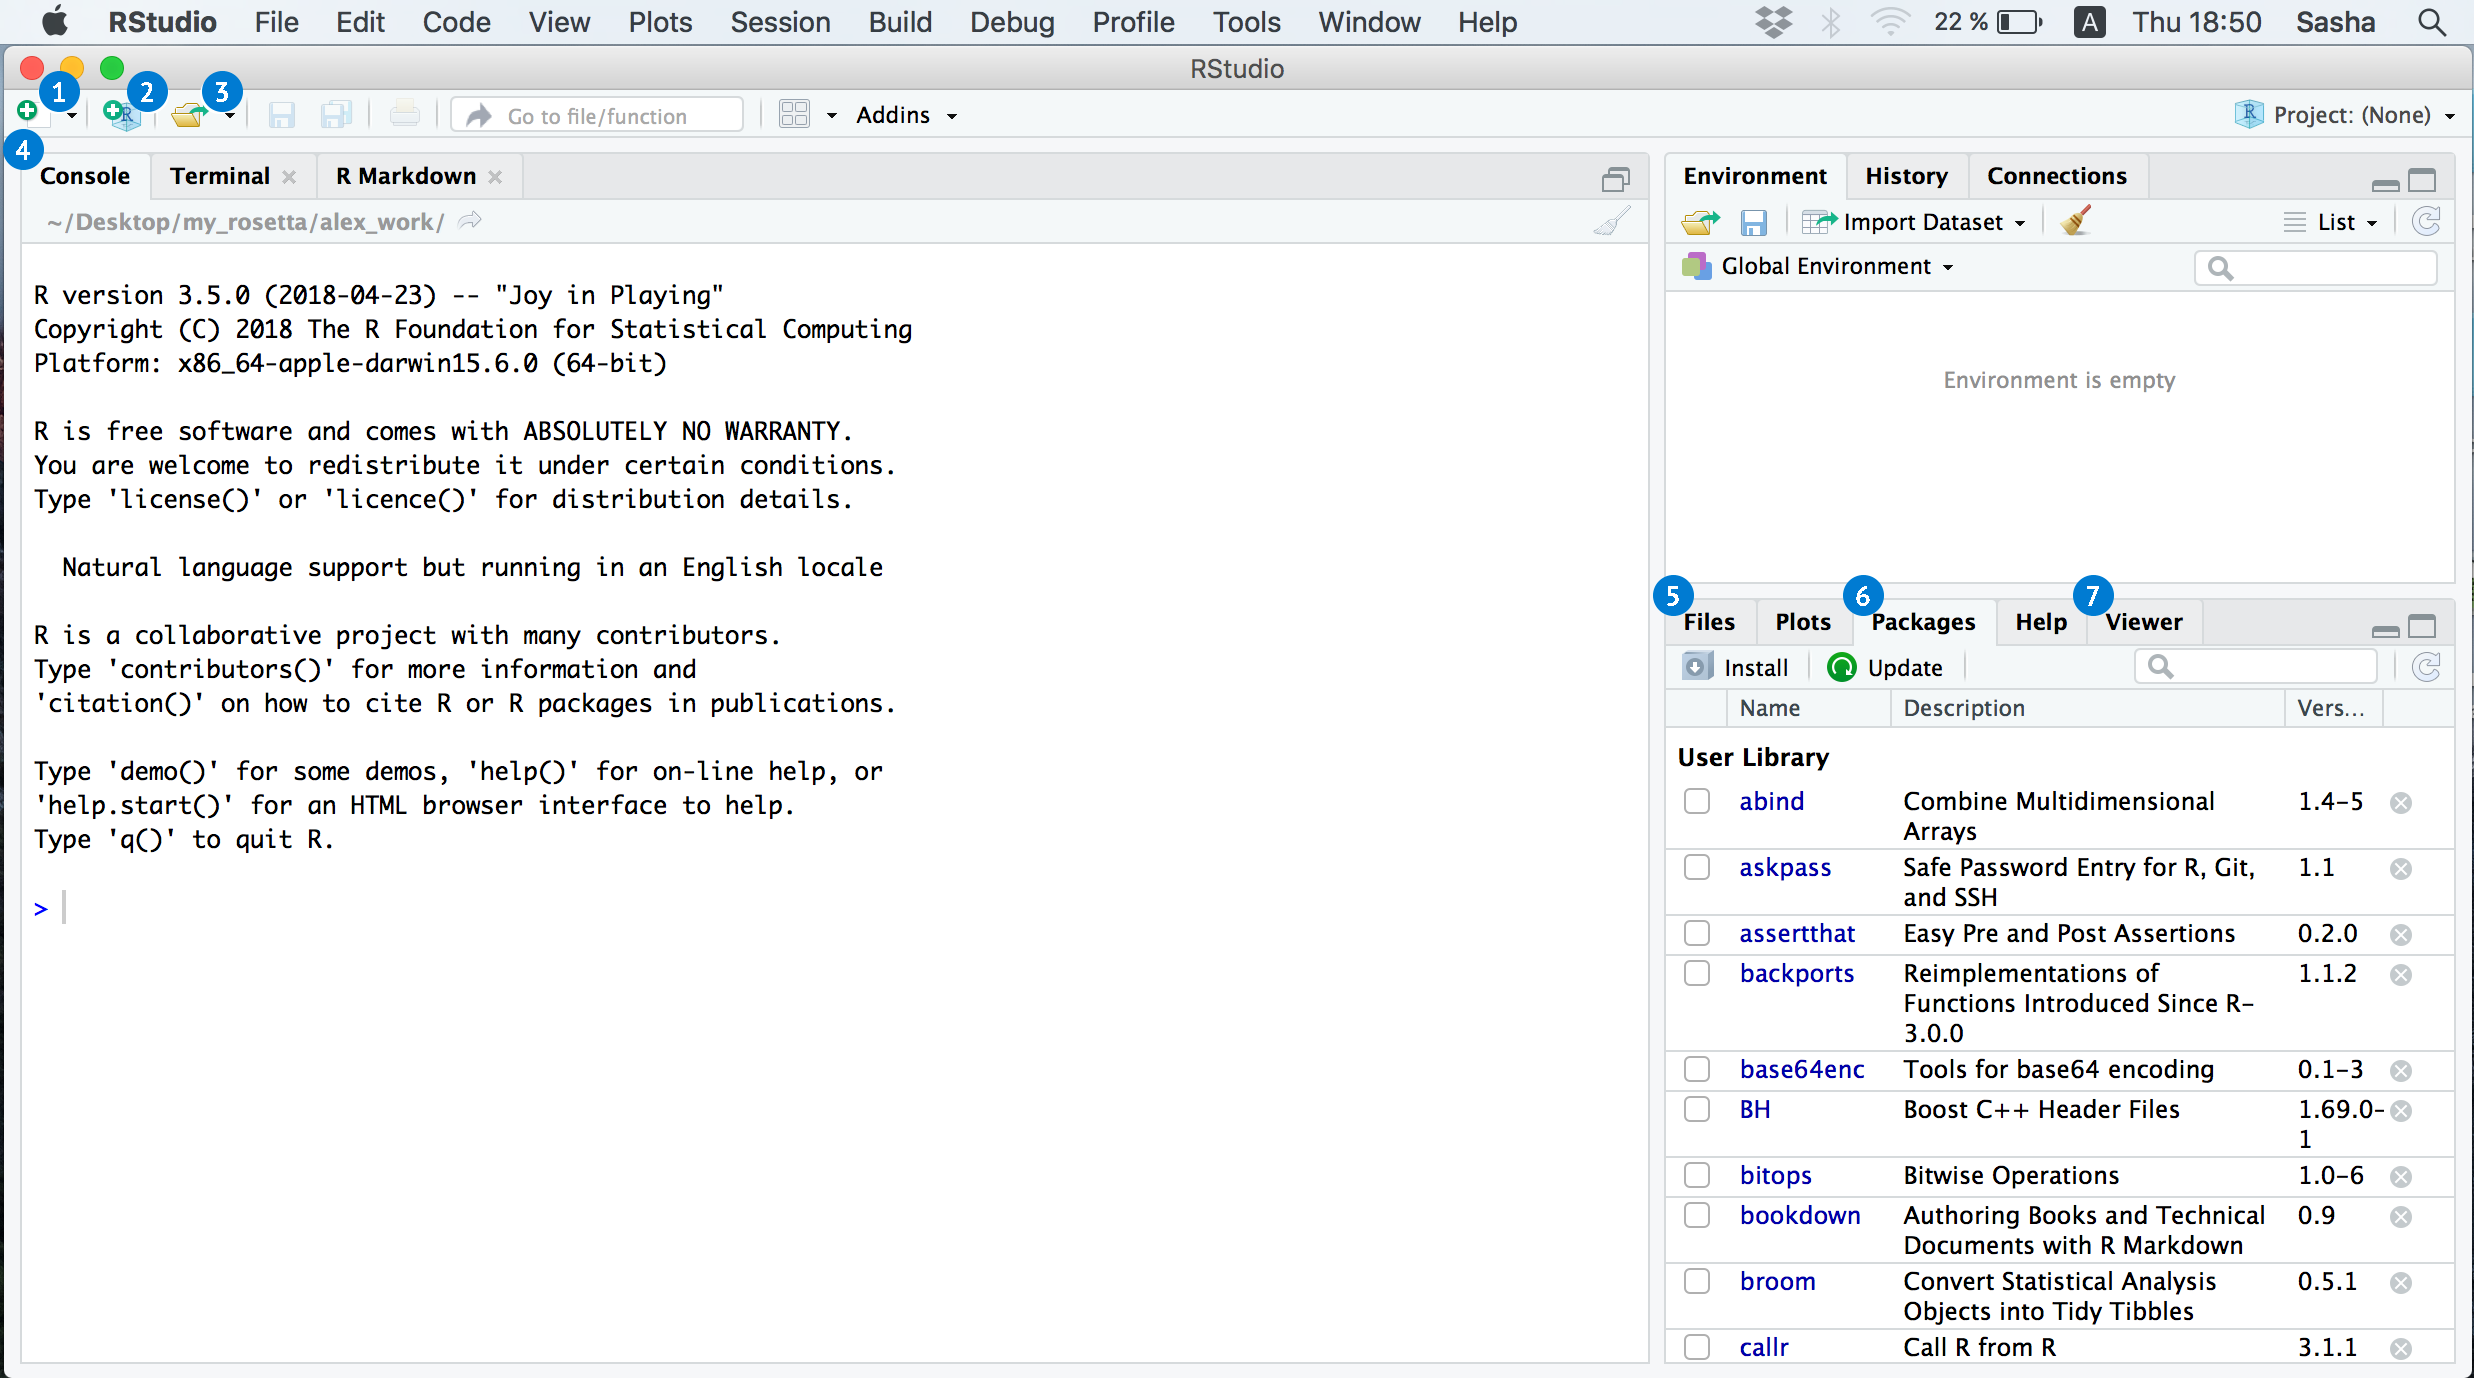
\includegraphics{images/RStudio_Interface.png}
\caption{\emph{Интерфейс программы}}
\end{figure}

\begin{enumerate}
\def\labelenumi{\arabic{enumi}.}
\item
  \textbf{New file} - Создание нового файла.
\item
  \textbf{New project} - Создание нового проекта.
\item
  \textbf{Open file} - Открытие существующего файла.
\item
  \textbf{Console} - Консоль, в которой набирается код.
\item
  \textbf{Files} - Список файлов, доступных для работы.
\item
  \textbf{Packages} - Список установленных пакетов, т.е. расширений. Также можно ознакомиться с ним, введя в консоль команду \emph{installed.packages()}.
\item
  \textbf{Viewer} - Отображение введенного кода.
\end{enumerate}

\begin{center}\rule{0.5\linewidth}{\linethickness}\end{center}

\#\#\#Язык программирования Python
\textgreater{} Python - это ещё одна открытая среда программирования, помогающая в работе со статистическими данными. Для программирования на Python подойдет программа Jupyter Notebook.

\#\#\#\#\#Установка

\begin{enumerate}
\def\labelenumi{\arabic{enumi}.}
\item
  Загрузите и установите Anaconda \href{https://www.anaconda.com/distribution/}{с официального сайта}.
\item
  После загрузки и установки откройте Anaconda Navigator, через который Вы сможете открыть программу Jupyter Notebook.
  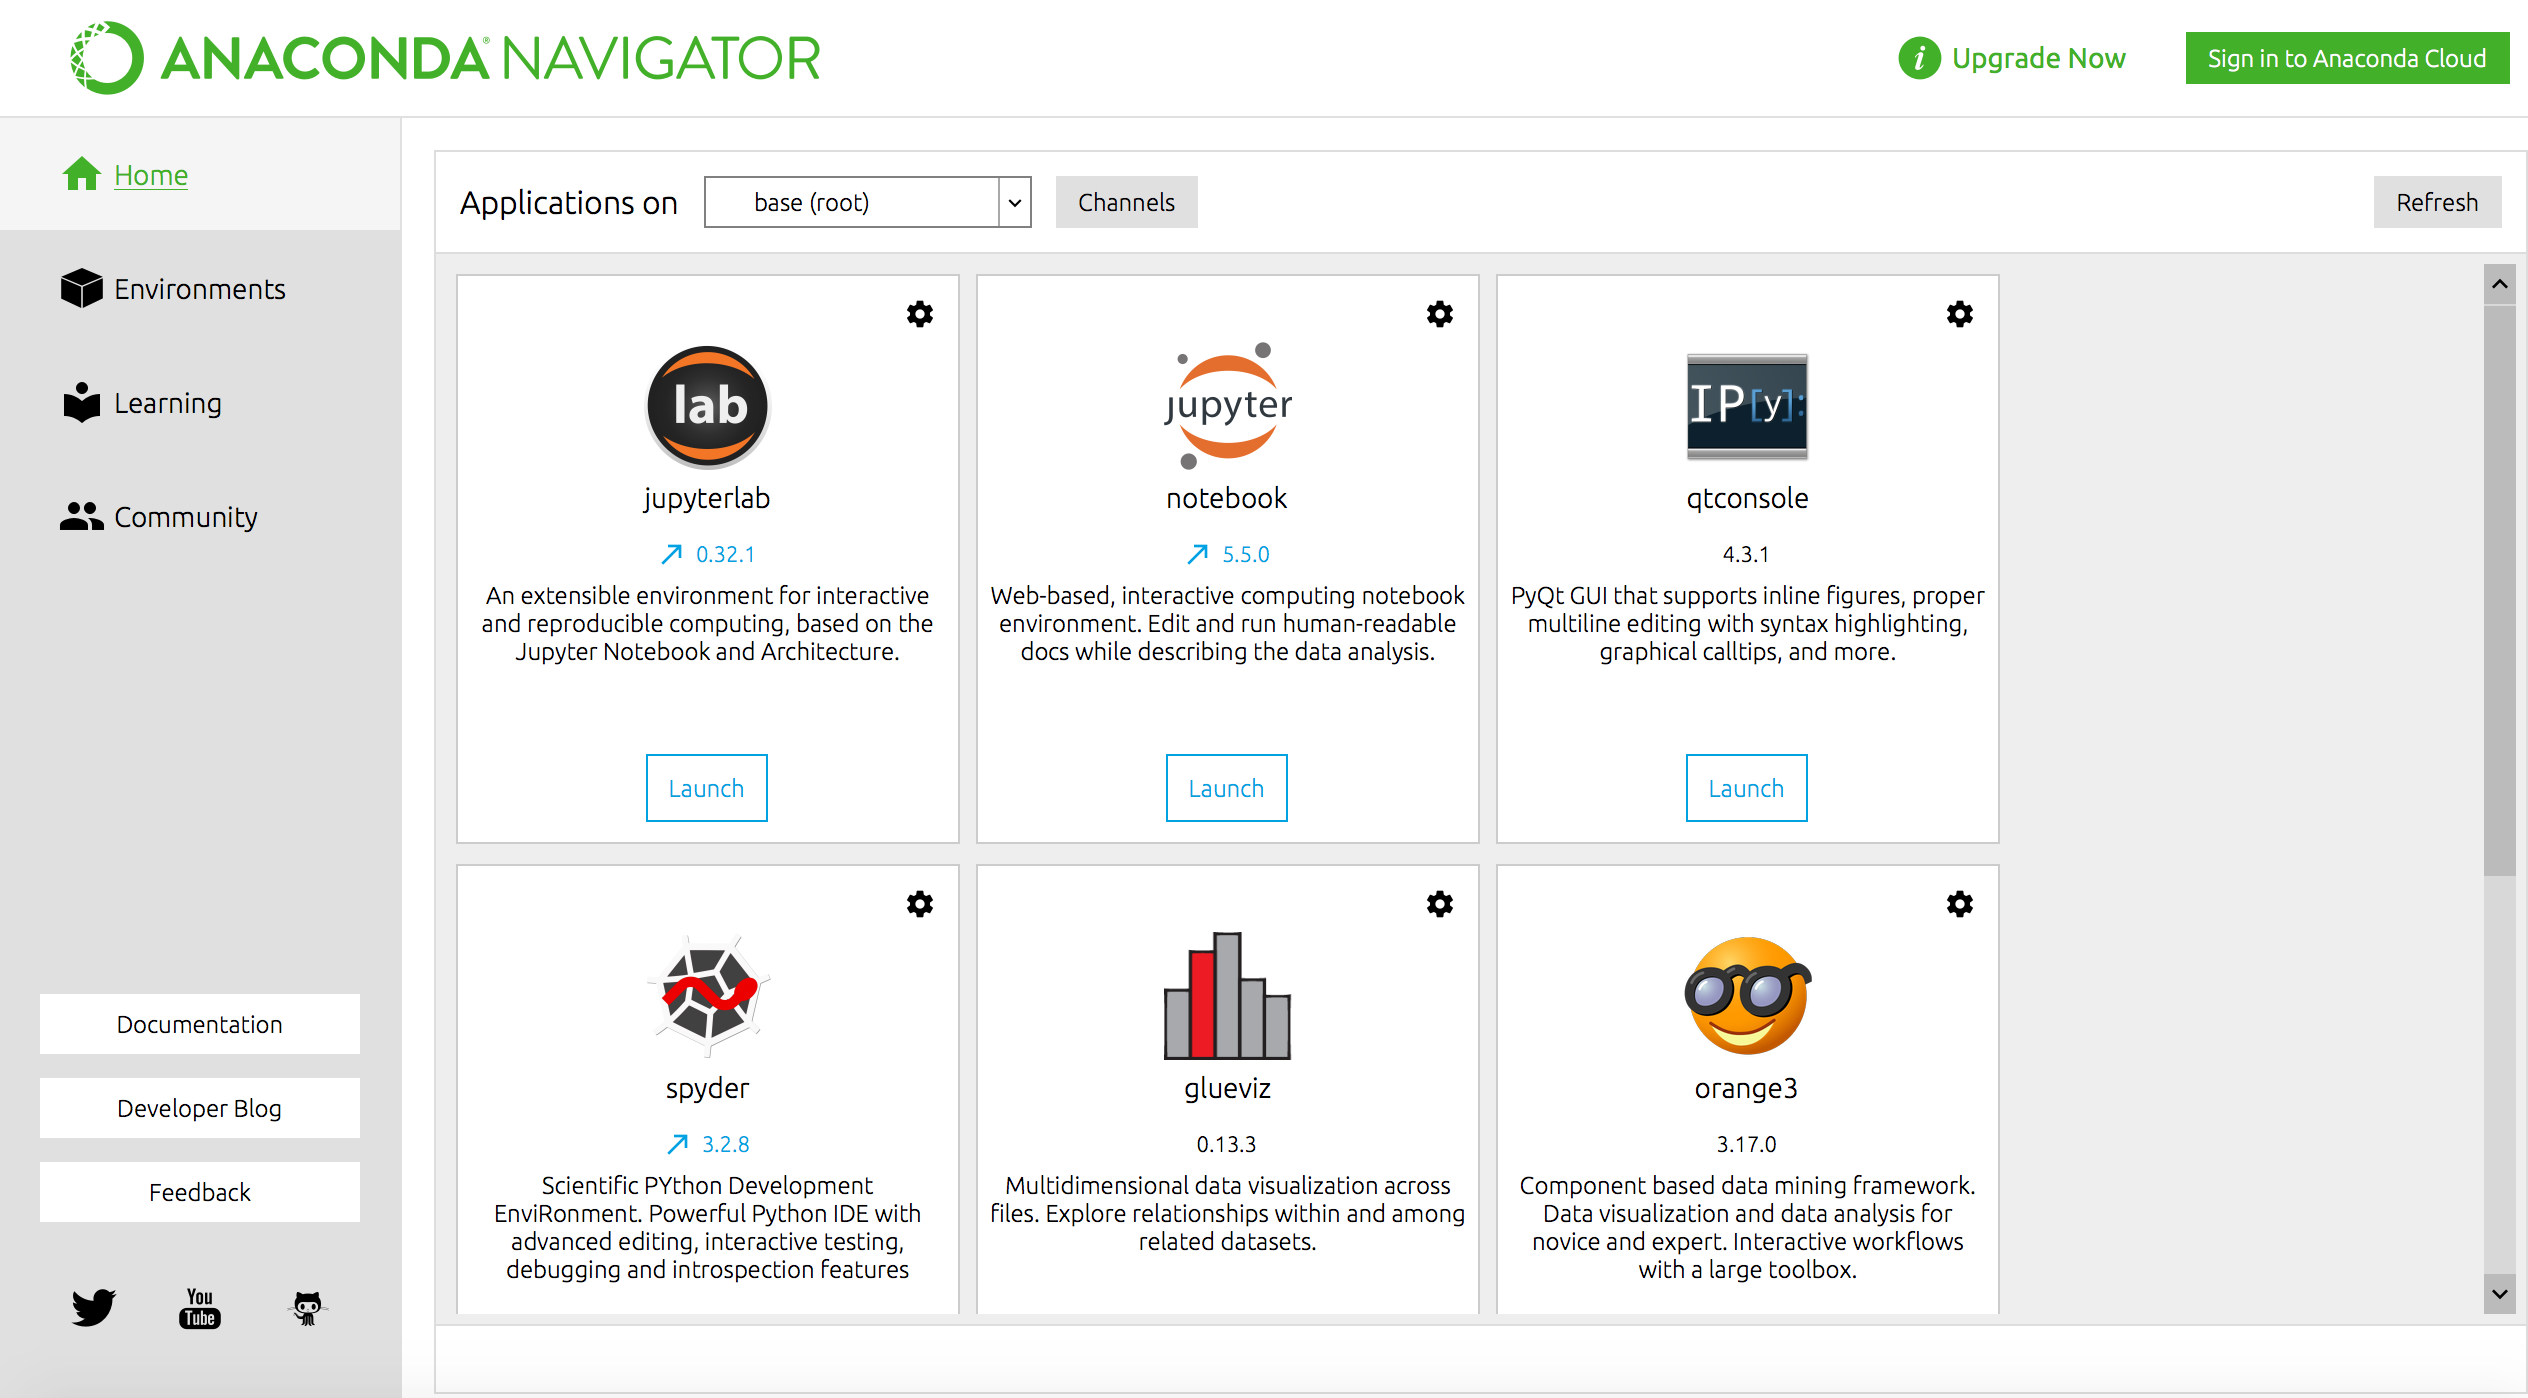
\includegraphics{images/Anaconda Navigator.png}
\end{enumerate}

\#\#\#\#\#Начало работы

Открыв Jupyter Notebook, вы попадете на страницу, содержащую ваши сохраненные файлы. Чтобы создать новый файл, нажмите ``New'' ▶ ``Notebook: Python 3''.
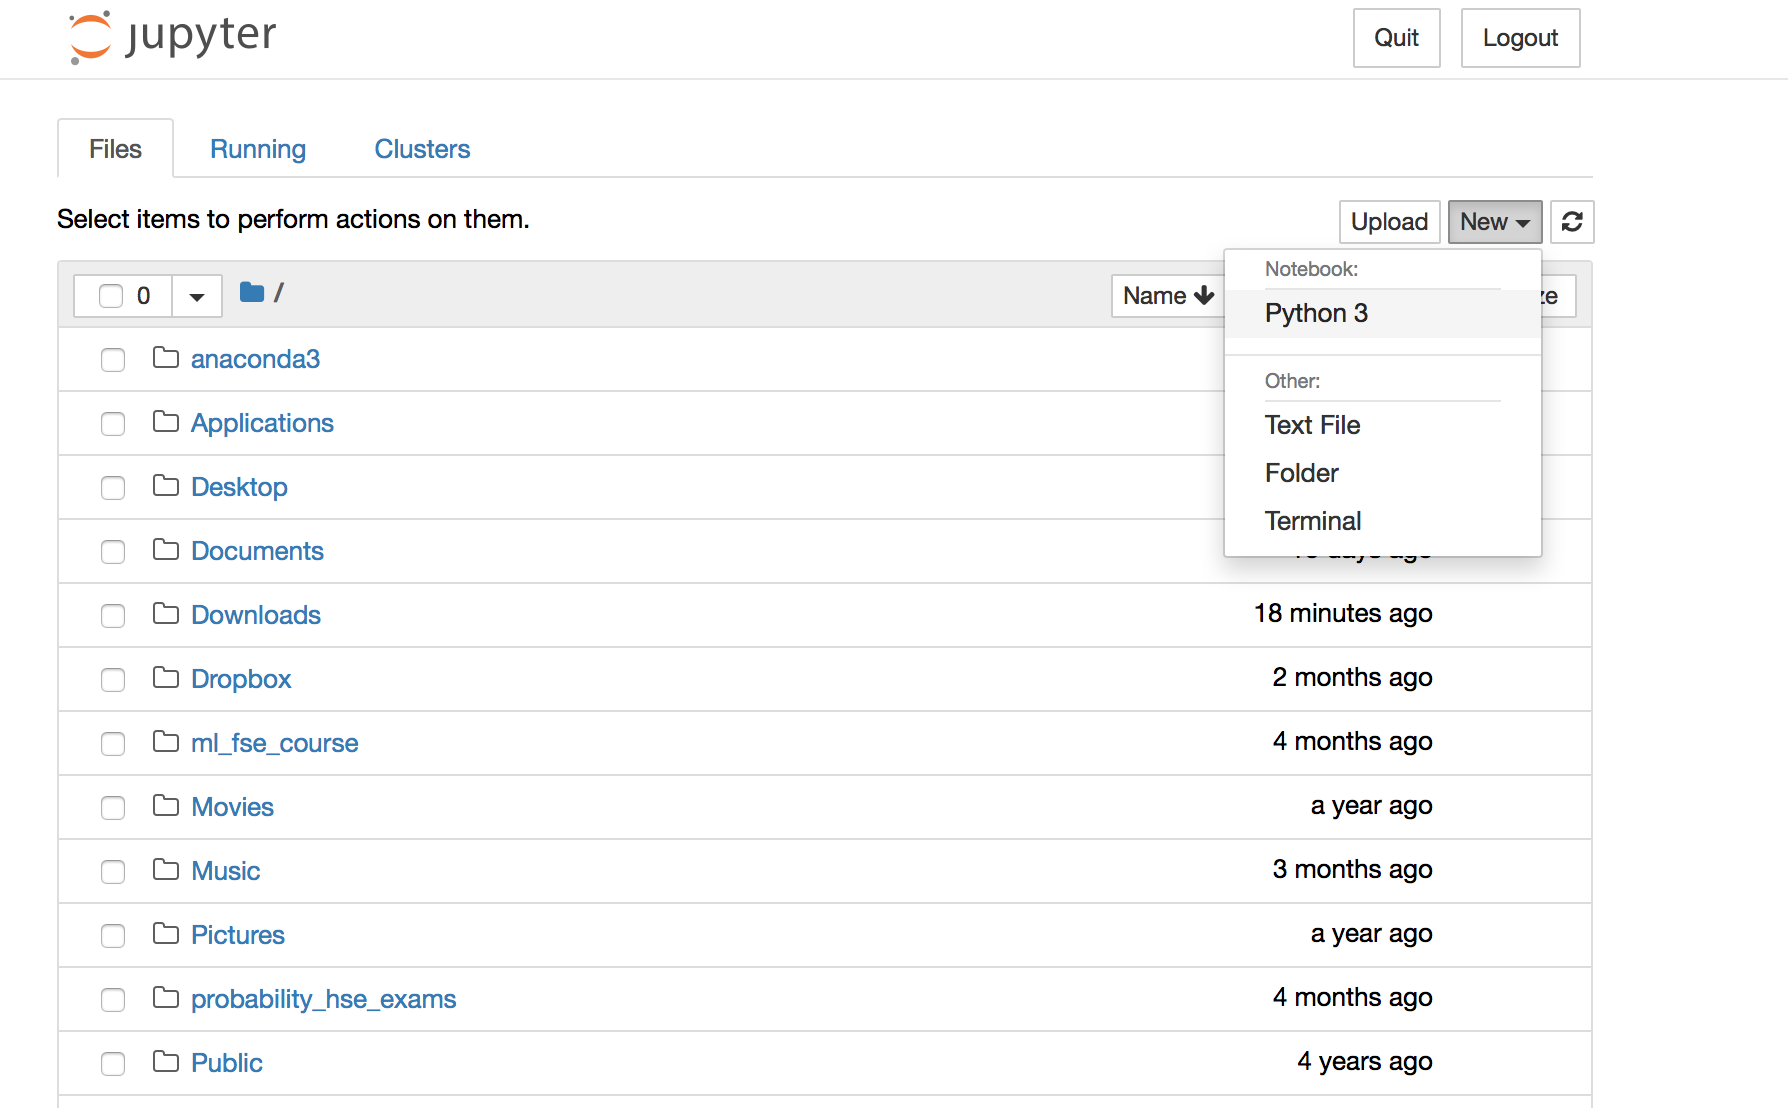
\includegraphics{images/New File in Jupyter.png}

Затем, в открывшемся окне, появится новый файл. Теперь все готово к работе. Вы можете вводить свой код и затем, используя комбинацию клавиш ``Shift'' + ``Enter'', проверять его исполнение.
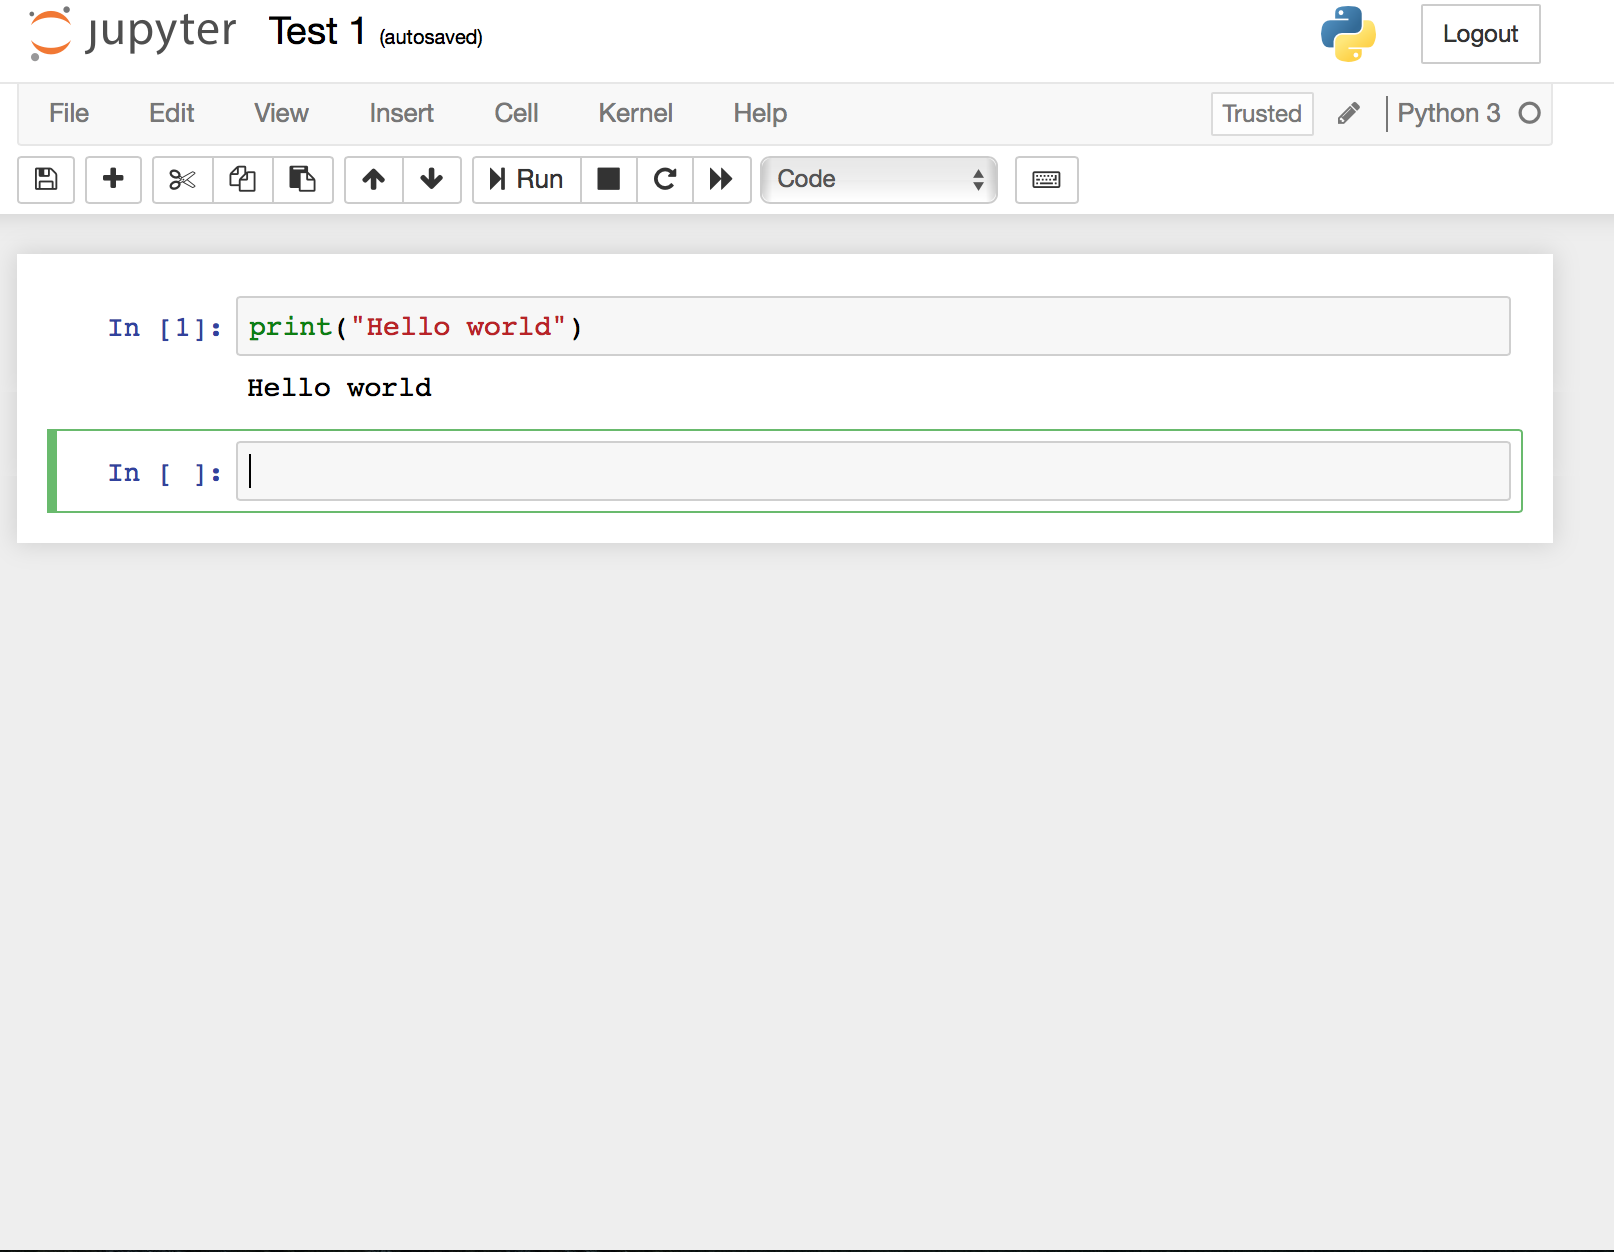
\includegraphics{images/Code in Jupyter.png}

\begin{center}\rule{0.5\linewidth}{\linethickness}\end{center}

\#\#\#Программа STATA
\textgreater{} Stata, в отличие от R и Python, является программой, а не языком программирования. Она также помогает в работе со статистическими данными.

\#\#\#\#\#Установка:

Для установки Stata необходимо загрузить актуальную версию \href{https://www.stata.com/}{с сайта компании-разработчика}. Подойдут как Stata SE, так и Stata MP.

\#\#\#\#\#Начало работы:

\begin{figure}
\centering
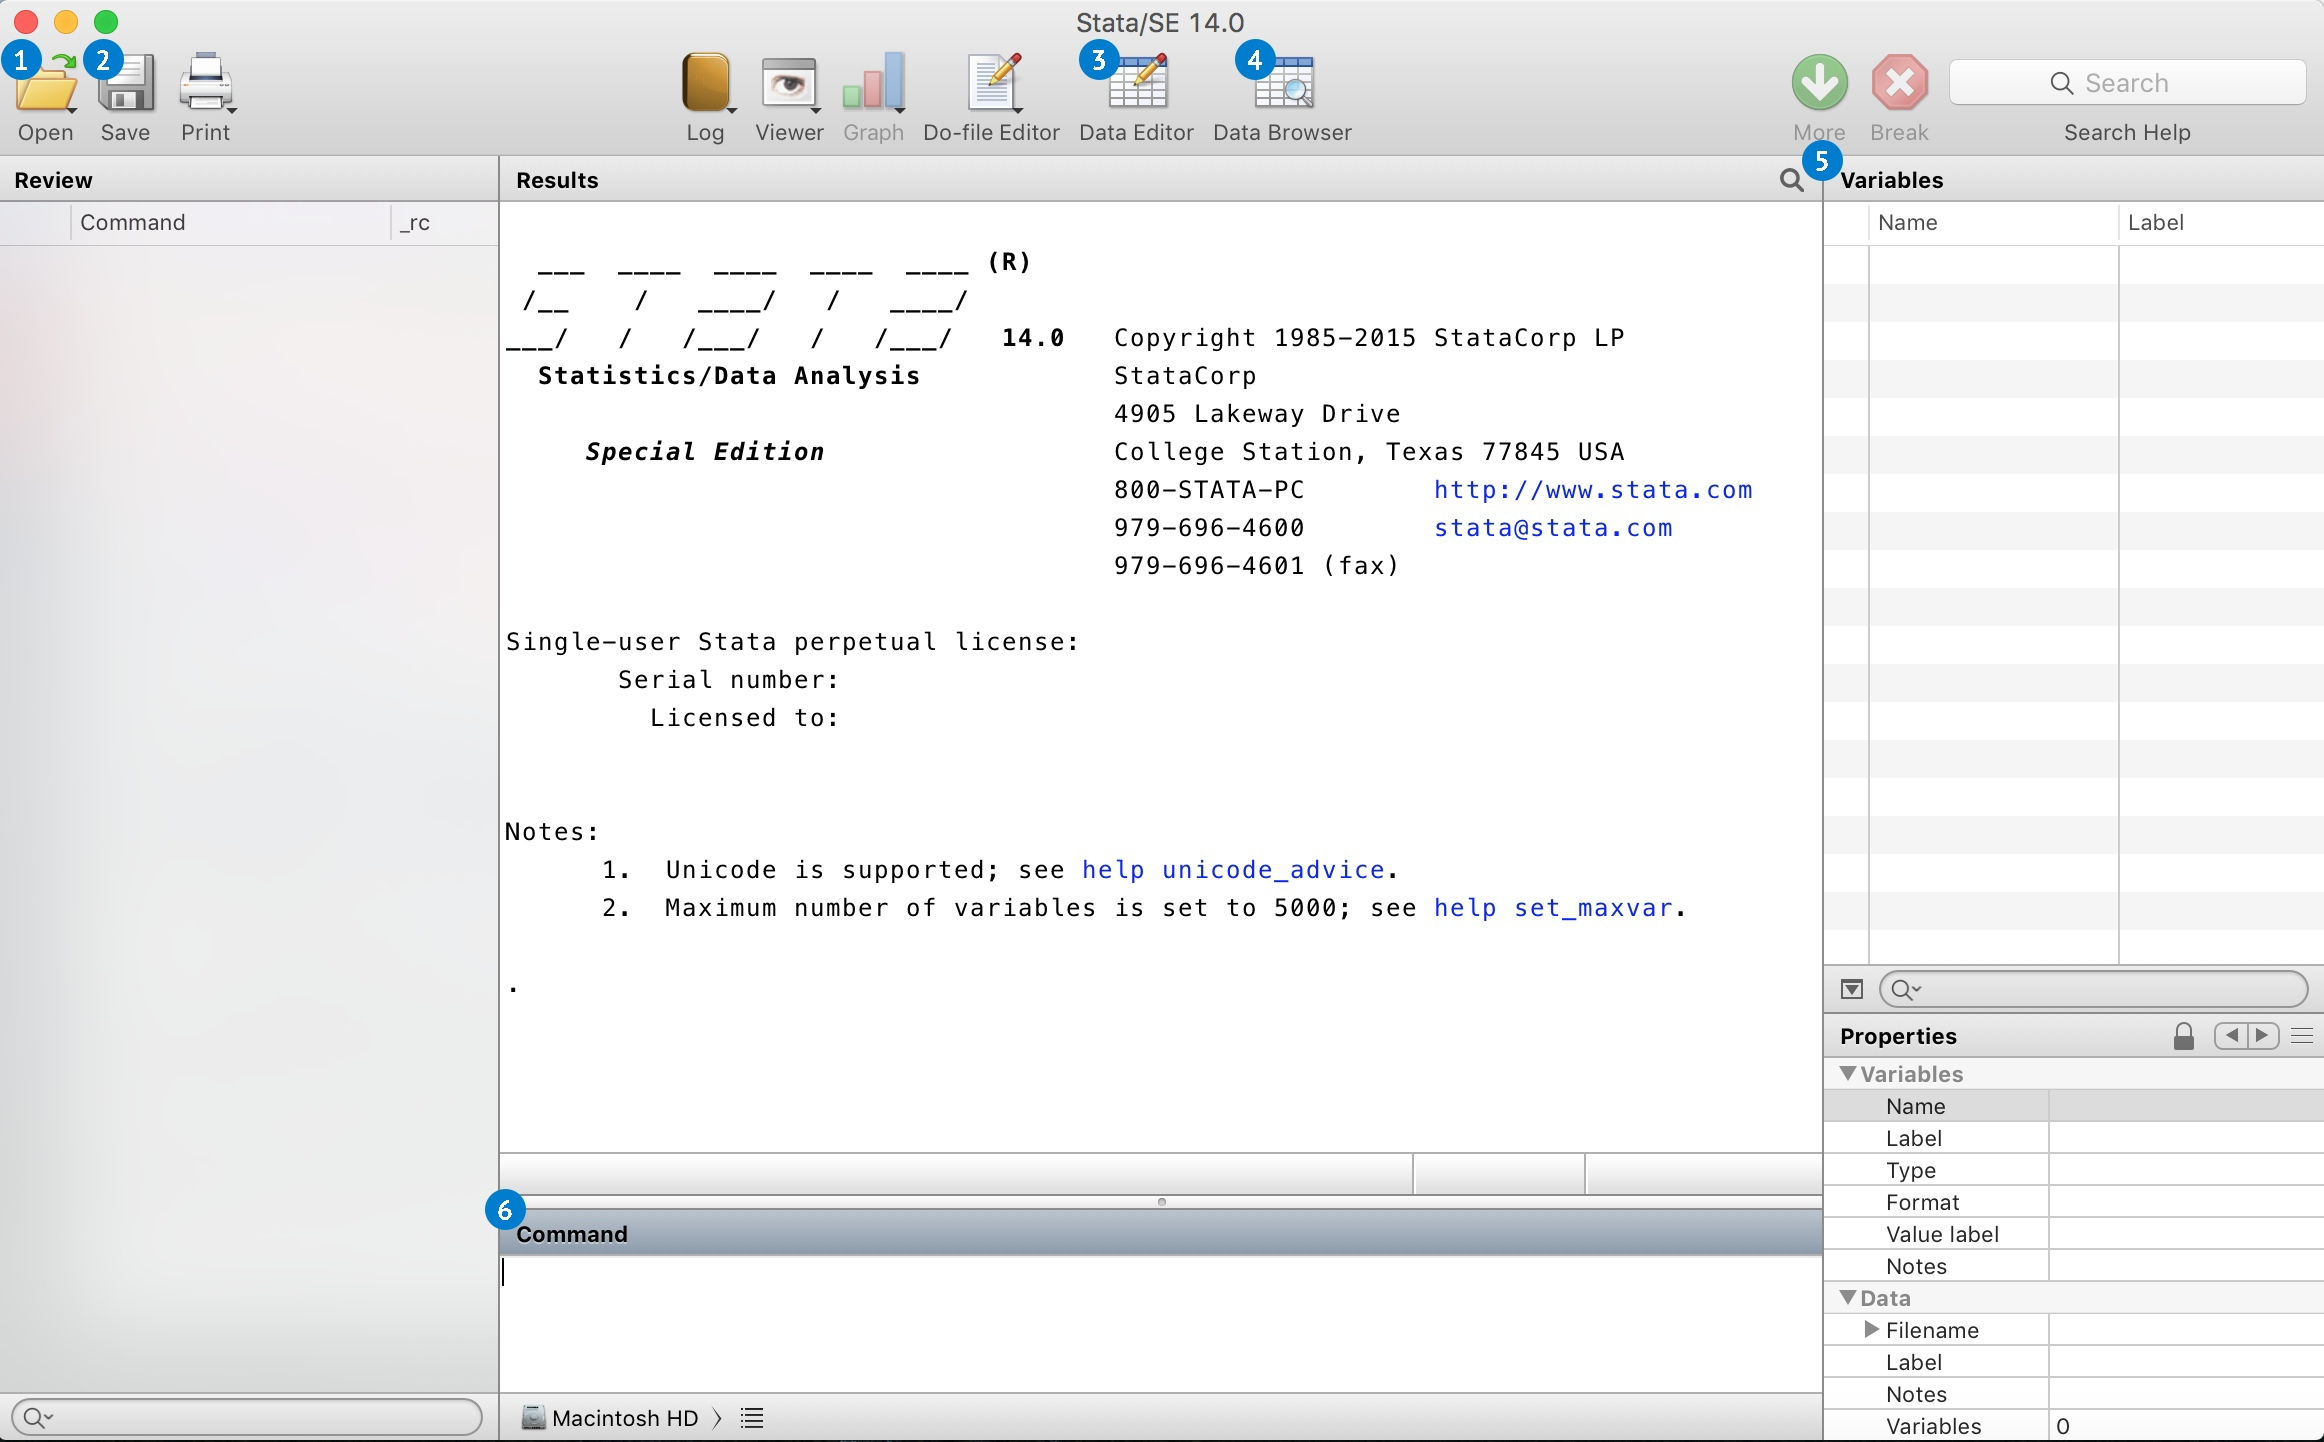
\includegraphics{images/Stata Interface.jpg}
\caption{\emph{Интерфейс Stata}}
\end{figure}

\begin{enumerate}
\def\labelenumi{\arabic{enumi}.}
\tightlist
\item
  \textbf{Open File} - открыть файл.
\item
  \textbf{Save} - сохранить файл.
\item
  \textbf{Data Editor} - редактирование данных.
\item
  \textbf{Data Browser} - просмотр данных.
\item
  \textbf{Variables} - список переменных.
\item
  \textbf{Command} - командная строка, в которой вводится код.
\end{enumerate}

\hypertarget{simplereg}{%
\chapter{Коан о простой линейной регрессии}\label{simplereg}}

Построим простую линейную регрессию в R и проведем несложные тесты.

Загрузим необходимые пакеты.

\begin{Shaded}
\begin{Highlighting}[]
\KeywordTok{library}\NormalTok{(tidyverse) }\CommentTok{# для манипуляций с данными и построения графиков}
\KeywordTok{library}\NormalTok{(skimr) }\CommentTok{# для красивого summary}
\KeywordTok{library}\NormalTok{(rio) }\CommentTok{# для чтения .dta файлов}
\KeywordTok{library}\NormalTok{(car) }\CommentTok{# для линейных гипотез}
\KeywordTok{library}\NormalTok{(tseries) }\CommentTok{# для теста на нормальность}
\KeywordTok{library}\NormalTok{(sjPlot) }\CommentTok{# еще графики}
\end{Highlighting}
\end{Shaded}

Импортируем данные.

\begin{Shaded}
\begin{Highlighting}[]
\NormalTok{df =}\StringTok{ }\KeywordTok{import}\NormalTok{(}\StringTok{"us-return.dta"}\NormalTok{)}
\end{Highlighting}
\end{Shaded}

Исследуем наш датасет.

\begin{Shaded}
\begin{Highlighting}[]
\CommentTok{# skim_with(numeric = list(hist = NULL, p25 = NULL, p75 = NULL)) # опустим некоторые описательные характеристики}
\KeywordTok{skim}\NormalTok{(df) }\CommentTok{# посмотрим на данные}
\end{Highlighting}
\end{Shaded}

\begin{verbatim}
Skim summary statistics
 n obs: 2664 
 n variables: 22 

-- Variable type:character -----------------------------------------------------------------------------------------------------------------------
 variable missing complete    n min max empty n_unique
        B       0     2664 2664   0   6  2544       31

-- Variable type:numeric -------------------------------------------------------------------------------------------------------------------------
 variable missing complete    n    mean      sd      p0     p25     p50
        A    2544      120 2664 60.5    34.79    1      30.75   60.5   
    BOISE    2544      120 2664  0.017   0.097  -0.27   -0.045   0.015 
   CITCRP    2544      120 2664  0.012   0.081  -0.28   -0.037   0.011 
    CONED    2544      120 2664  0.019   0.05   -0.14   -0.012   0.019 
   CONTIL    2544      120 2664 -0.0011  0.15   -0.6    -0.051   0     
   DATGEN    2544      120 2664  0.0075  0.13   -0.34   -0.072   0.017 
      DEC    2544      120 2664  0.02    0.099  -0.36   -0.051   0.024 
    DELTA    2544      120 2664  0.012   0.096  -0.26   -0.053   0.013 
   GENMIL    2544      120 2664  0.017   0.065  -0.15   -0.026   0.011 
   GERBER    2544      120 2664  0.016   0.088  -0.29   -0.036   0.015 
      IBM    2544      120 2664  0.0096  0.059  -0.19   -0.029   0.002 
   MARKET    2544      120 2664  0.014   0.068  -0.26   -0.013   0.012 
    MOBIL    2544      120 2664  0.016   0.08   -0.18   -0.032   0.013 
    MOTOR    2544      120 2664  0.018   0.097  -0.33   -0.053   0.017 
    PANAM    2544      120 2664  0.0035  0.13   -0.31   -0.065   0     
     PSNH    2544      120 2664 -0.0042  0.11   -0.48   -0.049   0     
   rkfree    2544      120 2664  0.0068  0.0022  0.0021  0.0052  0.0066
   RKFREE    2544      120 2664  0.0068  0.0022  0.0021  0.0052  0.0066
    TANDY    2544      120 2664  0.025   0.13   -0.25   -0.058   0.022 
   TEXACO    2544      120 2664  0.012   0.08   -0.19   -0.037   0.01  
    WEYER    2544      120 2664  0.0096  0.085  -0.27   -0.049  -0.002 
     p75    p100     hist
 90.25   120     ▇▇▇▇▇▇▇▇
  0.07     0.38  ▁▂▆▇▇▂▁▁
  0.064    0.32  ▁▁▅▇▇▃▁▁
  0.045    0.15  ▁▁▂▇▇▅▂▂
  0.058    0.97  ▁▁▇▇▁▁▁▁
  0.078    0.53  ▁▂▅▇▃▁▁▁
  0.075    0.39  ▁▁▂▇▇▂▁▁
  0.063    0.29  ▁▂▅▇▇▃▂▁
  0.06     0.19  ▁▃▅▇▅▃▂▁
  0.065    0.23  ▁▁▁▅▇▅▂▁
  0.05     0.15  ▁▁▂▇▇▆▃▂
  0.062    0.15  ▁▁▁▂▅▇▇▂
  0.057    0.37  ▁▃▇▇▂▁▁▁
  0.084    0.27  ▁▁▂▇▇▇▃▁
  0.074    0.41  ▁▂▅▇▃▁▁▁
  0.043    0.32  ▁▁▁▁▇▆▁▁
  0.0078   0.013 ▁▃▆▇▅▂▂▂
  0.0078   0.013 ▁▃▆▇▅▂▂▂
  0.094    0.45  ▂▃▆▇▂▂▁▁
  0.048    0.4   ▁▃▇▆▂▁▁▁
  0.06     0.27  ▁▁▅▇▆▃▂▁
\end{verbatim}

\begin{Shaded}
\begin{Highlighting}[]
\NormalTok{df =}\StringTok{ }\KeywordTok{rename}\NormalTok{(df, }\DataTypeTok{n =}\NormalTok{ A, }\DataTypeTok{date =}\NormalTok{ B) }\CommentTok{# дадим столбцам более осмысленные названия}
\end{Highlighting}
\end{Shaded}

\begin{Shaded}
\begin{Highlighting}[]
\NormalTok{df =}\StringTok{ }\KeywordTok{na.omit}\NormalTok{(df) }\CommentTok{# уберем строки с пропущенными наблюдениями}
\end{Highlighting}
\end{Shaded}

Будем верить в CAPM :) Оценим параметры модели для компании MOTOR. Соответственно, зависимая переменная - разница доходностей акций MOTOR и безрискового актива, а регрессор - рыночная премия.

\begin{Shaded}
\begin{Highlighting}[]
\CommentTok{#создаем новые переменные и добавляем их к набору данных}
\NormalTok{df =}\StringTok{ }\KeywordTok{mutate}\NormalTok{(df, }\DataTypeTok{y =}\NormalTok{ MOTOR }\OperatorTok{-}\StringTok{ }\NormalTok{RKFREE, }\DataTypeTok{x =}\NormalTok{ MARKET }\OperatorTok{-}\StringTok{ }\NormalTok{RKFREE) }
\end{Highlighting}
\end{Shaded}

Строим нашу модель и проверяем гипотезу об адекватности регрессии.

\begin{Shaded}
\begin{Highlighting}[]
\NormalTok{ols =}\StringTok{ }\KeywordTok{lm}\NormalTok{(y }\OperatorTok{~}\StringTok{ }\NormalTok{x, }\DataTypeTok{data =}\NormalTok{ df)}
\KeywordTok{summary}\NormalTok{(ols)}
\end{Highlighting}
\end{Shaded}

\begin{verbatim}

Call:
lm(formula = y ~ x, data = df)

Residuals:
      Min        1Q    Median        3Q       Max 
-0.168421 -0.059381 -0.003399  0.061373  0.182991 

Coefficients:
            Estimate Std. Error t value Pr(>|t|)    
(Intercept) 0.005253   0.007200   0.730    0.467    
x           0.848150   0.104814   8.092 5.91e-13 ***
---
Signif. codes:  0 '***' 0.001 '**' 0.01 '*' 0.05 '.' 0.1 ' ' 1

Residual standard error: 0.07844 on 118 degrees of freedom
Multiple R-squared:  0.3569,    Adjusted R-squared:  0.3514 
F-statistic: 65.48 on 1 and 118 DF,  p-value: 5.913e-13
\end{verbatim}

Вызовом одной функции получаем кучу полезных графиков. Можем визуально оценить наличие гетероскедастичности, нормальность распределения остатков, наличие выбросов.

\begin{Shaded}
\begin{Highlighting}[]
\KeywordTok{plot}\NormalTok{(ols)}
\end{Highlighting}
\end{Shaded}

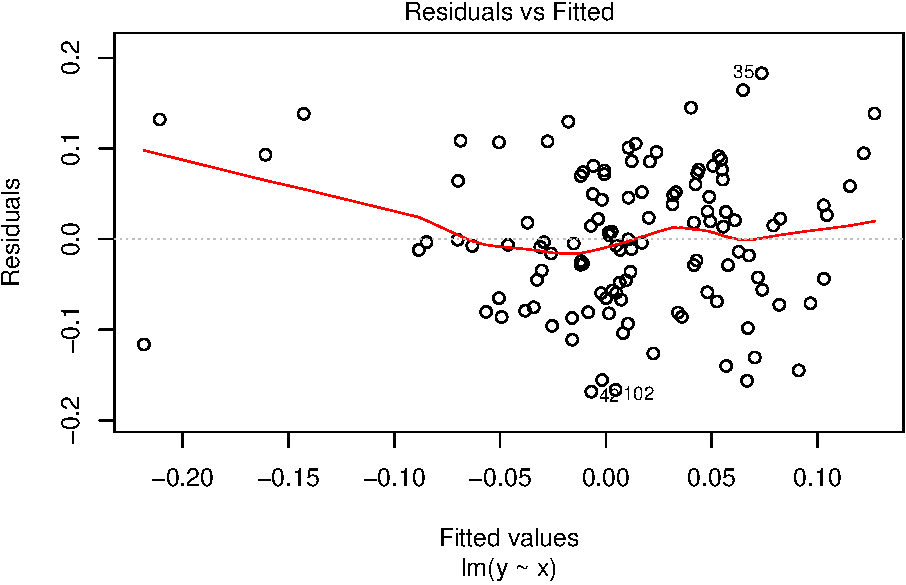
\includegraphics{02-simplereg_files/figure-latex/plot-1.pdf} 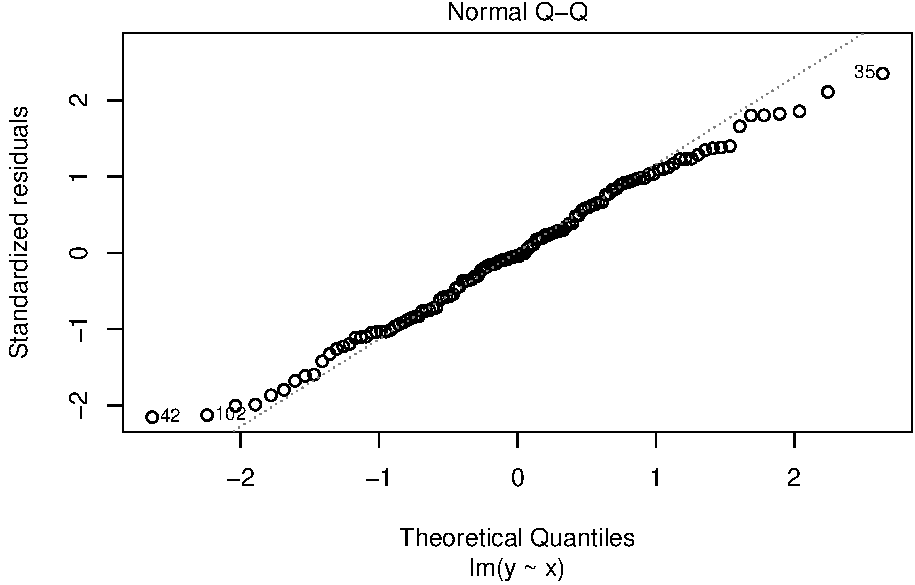
\includegraphics{02-simplereg_files/figure-latex/plot-2.pdf} 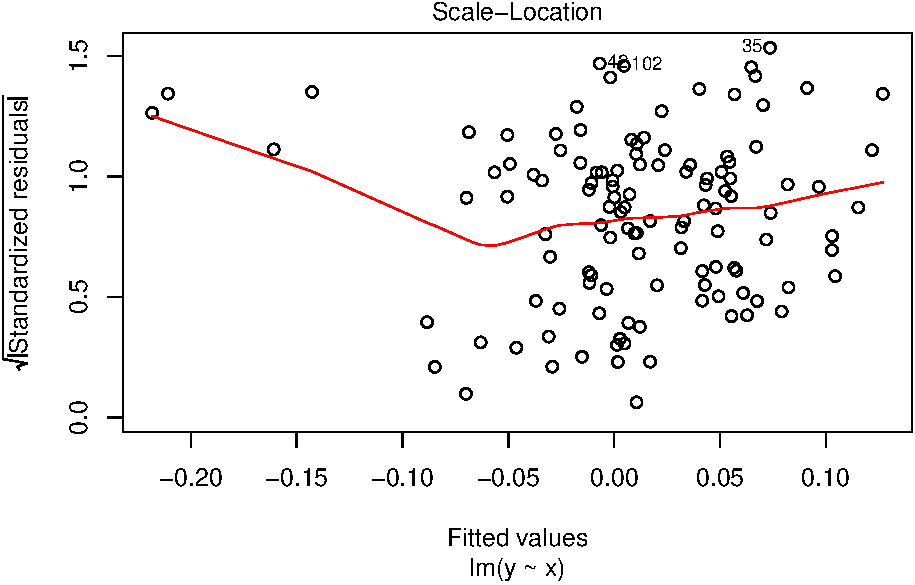
\includegraphics{02-simplereg_files/figure-latex/plot-3.pdf} 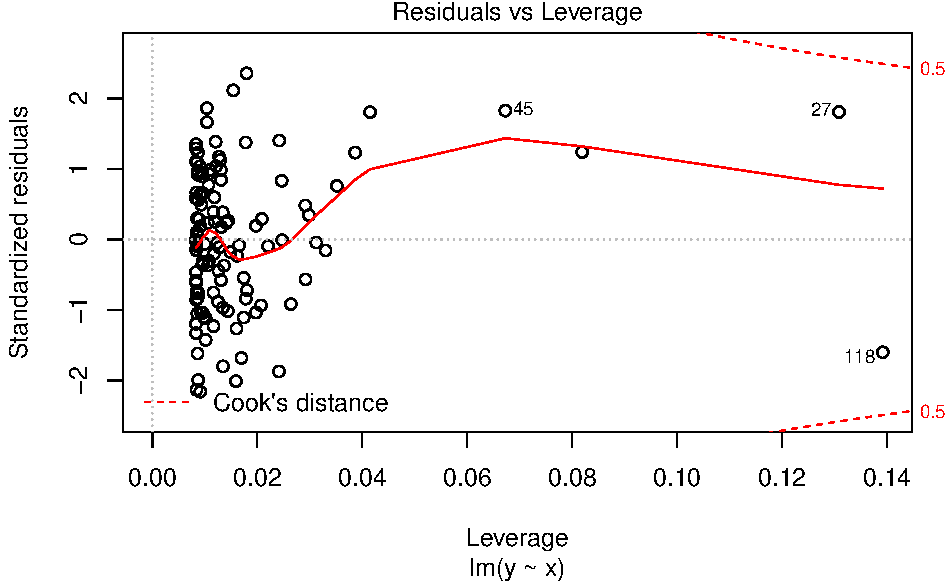
\includegraphics{02-simplereg_files/figure-latex/plot-4.pdf}

Строим доверительный интервал для параметров модели.

\begin{Shaded}
\begin{Highlighting}[]
\NormalTok{est =}\StringTok{ }\KeywordTok{cbind}\NormalTok{(}\DataTypeTok{Estimate =} \KeywordTok{coef}\NormalTok{(ols), }\KeywordTok{confint}\NormalTok{(ols))}
\end{Highlighting}
\end{Shaded}

Проверим гипотезу о равенстве коэффициента при регрессоре единице.

\begin{Shaded}
\begin{Highlighting}[]
\KeywordTok{linearHypothesis}\NormalTok{(ols, }\KeywordTok{c}\NormalTok{(}\StringTok{"x = 1"}\NormalTok{))}
\end{Highlighting}
\end{Shaded}

\begin{verbatim}
Linear hypothesis test

Hypothesis:
x = 1

Model 1: restricted model
Model 2: y ~ x

  Res.Df     RSS Df Sum of Sq      F Pr(>F)
1    119 0.73900                           
2    118 0.72608  1  0.012915 2.0989 0.1501
\end{verbatim}

Посмотрим на остатки :) Протестируем остатки регрессии на нормальность с помощью теста Харке-Бера.

\[
H_{0}: S = 0, K = 3,
\]
где \(S\) --- коэффициент асимметрии (Skewness), \(K\) --- коэффициент эксцесса (Kurtosis)

\begin{Shaded}
\begin{Highlighting}[]
\KeywordTok{jarque.bera.test}\NormalTok{(}\KeywordTok{resid}\NormalTok{(ols)) }
\end{Highlighting}
\end{Shaded}

\begin{verbatim}

    Jarque Bera Test

data:  resid(ols)
X-squared = 1.7803, df = 2, p-value = 0.4106
\end{verbatim}

И тест Шапиро-Уилка.

\(H_{0}: \epsilon_{i} \sim N(\mu,\sigma^2)\)

\begin{Shaded}
\begin{Highlighting}[]
\KeywordTok{shapiro.test}\NormalTok{(}\KeywordTok{resid}\NormalTok{(ols))}
\end{Highlighting}
\end{Shaded}

\begin{verbatim}

    Shapiro-Wilk normality test

data:  resid(ols)
W = 0.99021, p-value = 0.5531
\end{verbatim}

Оба теста указывают на нормальность распределения остатков регрессии.

Сделаем прогноз модели по данным вне обучаемой выборки.

\begin{Shaded}
\begin{Highlighting}[]
\KeywordTok{set.seed}\NormalTok{(}\DecValTok{7}\NormalTok{)}
\NormalTok{newData =}\StringTok{ }\NormalTok{df}
\NormalTok{newData =}\StringTok{ }\KeywordTok{mutate}\NormalTok{(newData, }\DataTypeTok{x =}\NormalTok{ x }\OperatorTok{+}\StringTok{ }\KeywordTok{rnorm}\NormalTok{(}\DataTypeTok{n =} \KeywordTok{n}\NormalTok{())) }\CommentTok{# пошумим}
\NormalTok{yhat =}\StringTok{ }\KeywordTok{predict}\NormalTok{(ols, }\DataTypeTok{newdata =}\NormalTok{ newData, }\DataTypeTok{se =} \OtherTok{TRUE}\NormalTok{)}
\end{Highlighting}
\end{Shaded}

\hypertarget{----}{%
\subsubsection{То же самое в стате}\label{----}}

Загружаем данные.

\begin{verbatim}
use us-return.dta
\end{verbatim}

\begin{verbatim}
end of do-file
\end{verbatim}

Любуемся и даем новые названия столбцам.

\begin{verbatim}
summarize
ren A n
ren B date
\end{verbatim}

\begin{verbatim}
    Variable |        Obs        Mean    Std. Dev.       Min        Max
-------------+---------------------------------------------------------
           A |        120        60.5    34.78505          1        120
           B |          0
       MOBIL |        120    .0161917    .0803075      -.178       .366
      TEXACO |        120    .0119417    .0797036      -.194       .399
         IBM |        120    .0096167     .059024      -.187        .15
-------------+---------------------------------------------------------
         DEC |        120      .01975    .0991438      -.364       .385
      DATGEN |        120    .0074833    .1275399      -.342       .528
       CONED |        120    .0185083    .0502719      -.139       .151
        PSNH |        120   -.0042167    .1094712      -.485       .318
       WEYER |        120    .0096333    .0850664      -.271        .27
-------------+---------------------------------------------------------
       BOISE |        120     .016675    .0974882      -.274       .379
       MOTOR |        120    .0181583    .0972656      -.331        .27
       TANDY |        120    .0250083     .127566      -.246       .454
       PANAM |        120    .0035167    .1318054      -.313       .406
       DELTA |        120    .0116917    .0959317       -.26       .289
-------------+---------------------------------------------------------
      CONTIL |        120      -.0011    .1506992        -.6       .974
      CITCRP |        120    .0118583    .0809719      -.282       .318
      GERBER |        120       .0164    .0877379      -.288       .234
      GENMIL |        120    .0165833    .0650403      -.148        .19
      MARKET |        120    .0139917    .0683532       -.26       .148
-------------+---------------------------------------------------------
      RKFREE |        120    .0068386    .0021869     .00207     .01255
      rkfree |        120    .0068386    .0021869     .00207     .01255
\end{verbatim}

Убираем пропущенные значения и создаем новые переменные.

\begin{verbatim}
drop if n == .
gen y = MOTOR - RKFREE
gen x = MARKET - RKFREE
\end{verbatim}

\begin{verbatim}
(2,544 observations deleted)
\end{verbatim}

Строим модель и проверяем гипотезу об адекватности регрессии. Тут же получаем доверительные интервалы для коэффициентов.

\begin{verbatim}
reg y x
\end{verbatim}

\begin{verbatim}
      Source |       SS           df       MS      Number of obs   =       120
-------------+----------------------------------   F(1, 118)       =     65.48
       Model |  .402913404         1  .402913404   Prob > F        =    0.0000
    Residual |  .726081541       118  .006153233   R-squared       =    0.3569
-------------+----------------------------------   Adj R-squared   =    0.3514
       Total |  1.12899494       119  .009487352   Root MSE        =    .07844

------------------------------------------------------------------------------
           y |      Coef.   Std. Err.      t    P>|t|     [95% Conf. Interval]
-------------+----------------------------------------------------------------
           x |   .8481496   .1048138     8.09   0.000     .6405898    1.055709
       _cons |   .0052529   .0071999     0.73   0.467     -.009005    .0195107
------------------------------------------------------------------------------
\end{verbatim}

Проверим гипотезу о равенстве коэффициента при регрессоре единице.

\begin{verbatim}
test x = 1
\end{verbatim}

\begin{verbatim}
 ( 1)  x = 1

       F(  1,   118) =    2.10
            Prob > F =    0.1501
\end{verbatim}

Сделаем предсказание по выборке и сохраним остатки.

\begin{verbatim}
predict u_hat, resid
predict y_hat
\end{verbatim}

\begin{verbatim}
(option xb assumed; fitted values)
\end{verbatim}

Протестируем остатки регрессии на нормальность с помощью теста Харке-Бера.
На самом деле, это не совсем тест Харке-Бера. Оригинальный вариант ассимптотический и в нем нет поправки на размер выборки. В Stata есть. Подробнее здесь \url{https://www.stata.com/manuals13/rsktest.pdf}

\begin{verbatim}
sktest u_hat
\end{verbatim}

\begin{verbatim}
                    Skewness/Kurtosis tests for Normality
                                                          ------ joint ------
    Variable |        Obs  Pr(Skewness)  Pr(Kurtosis) adj chi2(2)   Prob>chi2
-------------+---------------------------------------------------------------
       u_hat |        120     0.8841        0.1027        2.74         0.2539
\end{verbatim}

И тест Шапиро-Уилка. Тут все аналогично R.

\begin{verbatim}
swilk u_hat
\end{verbatim}

\begin{verbatim}
                   Shapiro-Wilk W test for normal data

    Variable |        Obs       W           V         z       Prob>z
-------------+------------------------------------------------------
       u_hat |        120    0.99021      0.942    -0.133    0.55310
\end{verbatim}

Гипотеза о нормальности остатков не отвергается.

QQ - график

\begin{verbatim}
qnorm u_hat 
\end{verbatim}

\begin{verbatim}

График предсказанных значений против остатков.

```stata
rvfplot, yline(0)
```
\end{verbatim}

График диагональных элементов матрицы-шляпницы против квадрата остатков (по сравнению с R оси поменялись местами).

\begin{verbatim}
lvr2plot
\end{verbatim}

``````

График предсказанных значений против стандартизиованных остатков. Размер точек на графике зависит от расстояния Кука для данного наблюдения.

\begin{verbatim}
predict D, cooksd
predict standard, rstandard

graph twoway scatter standard y_hat [aweight=D], msymbol(oh) yline(0)
\end{verbatim}

\begin{verbatim}
\end{verbatim}

\begin{verbatim}
set seed 7

set obs 120
gen x_new = x+ 0.5 *rnormal()
gen y_hat_new =  .8481496 * x_new+ .0052529
\end{verbatim}

\begin{verbatim}
number of observations (_N) was 120, now 120
\end{verbatim}

\hypertarget{----python}{%
\subsubsection{То же самое в python}\label{----python}}

Много хорошихх функций для статистических расчетов можно найти в пакете Statsmodels.

\begin{Shaded}
\begin{Highlighting}[]

\ImportTok{import}\NormalTok{ pandas }\ImportTok{as}\NormalTok{ pd }\CommentTok{# для работы с таблицами}
\ImportTok{import}\NormalTok{ numpy }\ImportTok{as}\NormalTok{ np }\CommentTok{# математика, работа с матрицами}
\ImportTok{import}\NormalTok{ matplotlib.pyplot }\ImportTok{as}\NormalTok{ plt }\CommentTok{# графики}
\ImportTok{import}\NormalTok{ statsmodels.api }\ImportTok{as}\NormalTok{ sm}
\ImportTok{import}\NormalTok{ statsmodels.formula.api }\ImportTok{as}\NormalTok{ smf}
\ImportTok{import}\NormalTok{ statsmodels.graphics.gofplots }\ImportTok{as}\NormalTok{ gf}
\ImportTok{from}\NormalTok{ statsmodels.stats.outliers_influence }\ImportTok{import}\NormalTok{ summary_table}
\ImportTok{import}\NormalTok{ seaborn }\ImportTok{as}\NormalTok{ sns }\CommentTok{# еще более классные графики}
\ImportTok{from}\NormalTok{ scipy.stats }\ImportTok{import}\NormalTok{ shapiro }\CommentTok{# еще математика}
\ImportTok{import}\NormalTok{ statsmodels.discrete.discrete_model}
\end{Highlighting}
\end{Shaded}

При желании, можем кастомизировать графики :)

\begin{Shaded}
\begin{Highlighting}[]
\NormalTok{plt.style.use(}\StringTok{'seaborn'}\NormalTok{)}
\NormalTok{plt.rc(}\StringTok{'font'}\NormalTok{, size}\OperatorTok{=}\DecValTok{14}\NormalTok{)}
\NormalTok{plt.rc(}\StringTok{'figure'}\NormalTok{, titlesize}\OperatorTok{=}\DecValTok{15}\NormalTok{)}
\NormalTok{plt.rc(}\StringTok{'axes'}\NormalTok{, labelsize}\OperatorTok{=}\DecValTok{15}\NormalTok{)}
\NormalTok{plt.rc(}\StringTok{'axes'}\NormalTok{, titlesize}\OperatorTok{=}\DecValTok{15}\NormalTok{)}
\end{Highlighting}
\end{Shaded}

Загрузим данные.

\begin{Shaded}
\begin{Highlighting}[]
\NormalTok{df }\OperatorTok{=}\NormalTok{ pd.read_stata(}\StringTok{'us-return.dta'}\NormalTok{)}
\end{Highlighting}
\end{Shaded}

Избавимся от наблюдений с пропущенными значенями.

\begin{Shaded}
\begin{Highlighting}[]
\NormalTok{df.dropna(inplace}\OperatorTok{=}\VariableTok{True}\NormalTok{) }\CommentTok{##ИСПРАВИТЬ (выкинуть только пропуски целевой и объяснющей)}
\NormalTok{df.reset_index(drop}\OperatorTok{=}\VariableTok{True}\NormalTok{, inplace}\OperatorTok{=}\VariableTok{True}\NormalTok{)}
\end{Highlighting}
\end{Shaded}

Переименуем столбцы.

\begin{Shaded}
\begin{Highlighting}[]
\NormalTok{df }\OperatorTok{=}\NormalTok{ df.rename(columns}\OperatorTok{=}\NormalTok{\{}\StringTok{'A'}\NormalTok{:}\StringTok{'n'}\NormalTok{, }\StringTok{'B'}\NormalTok{: }\StringTok{'date'}\NormalTok{\})}
\end{Highlighting}
\end{Shaded}

\begin{Shaded}
\begin{Highlighting}[]
\NormalTok{df[}\StringTok{'y'}\NormalTok{] }\OperatorTok{=}\NormalTok{ df[}\StringTok{'MOTOR'}\NormalTok{] }\OperatorTok{-}\NormalTok{ df[}\StringTok{'RKFREE'}\NormalTok{]}
\NormalTok{df[}\StringTok{'x'}\NormalTok{] }\OperatorTok{=}\NormalTok{ df[}\StringTok{'MARKET'}\NormalTok{] }\OperatorTok{-}\NormalTok{ df[}\StringTok{'RKFREE'}\NormalTok{] }
\end{Highlighting}
\end{Shaded}

Строим модель и читаем саммари :)

\begin{Shaded}
\begin{Highlighting}[]
\NormalTok{regr }\OperatorTok{=}\NormalTok{ smf.ols(}\StringTok{'y~x'}\NormalTok{, data }\OperatorTok{=}\NormalTok{ df).fit()}
\NormalTok{regr.summary()}
\end{Highlighting}
\end{Shaded}

\begin{verbatim}
<class 'statsmodels.iolib.summary.Summary'>
"""
                            OLS Regression Results                            
==============================================================================
Dep. Variable:                      y   R-squared:                       0.357
Model:                            OLS   Adj. R-squared:                  0.351
Method:                 Least Squares   F-statistic:                     65.48
Date:                 Пн, 16 сен 2019   Prob (F-statistic):           5.91e-13
Time:                        11:15:11   Log-Likelihood:                 136.18
No. Observations:                 120   AIC:                            -268.4
Df Residuals:                     118   BIC:                            -262.8
Df Model:                           1                                         
Covariance Type:            nonrobust                                         
==============================================================================
                 coef    std err          t      P>|t|      [0.025      0.975]
------------------------------------------------------------------------------
Intercept      0.0053      0.007      0.730      0.467      -0.009       0.020
x              0.8481      0.105      8.092      0.000       0.641       1.056
==============================================================================
Omnibus:                        2.684   Durbin-Watson:                   2.030
Prob(Omnibus):                  0.261   Jarque-Bera (JB):                1.780
Skew:                          -0.031   Prob(JB):                        0.411
Kurtosis:                       2.406   Cond. No.                         14.6
==============================================================================

Warnings:
[1] Standard Errors assume that the covariance matrix of the errors is correctly specified.
"""
\end{verbatim}

Получить прогноз.

\begin{Shaded}
\begin{Highlighting}[]
\NormalTok{df[}\StringTok{'yhat'}\NormalTok{] }\OperatorTok{=}\NormalTok{ regr.fittedvalues}
\end{Highlighting}
\end{Shaded}

Красивые графики для остатков, выборосов и прочих радостей, как в R, придется строить ручками. Зато приятно поиграть с оформлением :)

\begin{Shaded}
\begin{Highlighting}[]
\NormalTok{fig, ax }\OperatorTok{=}\NormalTok{ plt.subplots()}
\NormalTok{ax.plot(df[}\StringTok{'x'}\NormalTok{],regr.fittedvalues, color}\OperatorTok{=}\StringTok{'g'}\NormalTok{, alpha }\OperatorTok{=}\FloatTok{0.8}\NormalTok{)}
\NormalTok{ax.scatter(df[}\StringTok{'x'}\NormalTok{],regr.fittedvalues}\OperatorTok{+}\NormalTok{regr.resid, color }\OperatorTok{=} \StringTok{'g'}\NormalTok{, alpha }\OperatorTok{=} \FloatTok{0.8}\NormalTok{, s }\OperatorTok{=} \DecValTok{40}\NormalTok{)}
\NormalTok{ax.vlines(df[}\StringTok{'x'}\NormalTok{],regr.fittedvalues,regr.fittedvalues}\OperatorTok{+}\NormalTok{regr.resid, color }\OperatorTok{=} \StringTok{'gray'}\NormalTok{, alpha }\OperatorTok{=} \FloatTok{0.5}\NormalTok{)}
\NormalTok{plt.title(}\StringTok{'Линия регрессии и остатки'}\NormalTok{)}
\NormalTok{plt.xlabel(}\StringTok{'RKFREE'}\NormalTok{)}
\NormalTok{plt.ylabel(}\StringTok{'MARKET'}\NormalTok{)}
\NormalTok{plt.show()}
\end{Highlighting}
\end{Shaded}

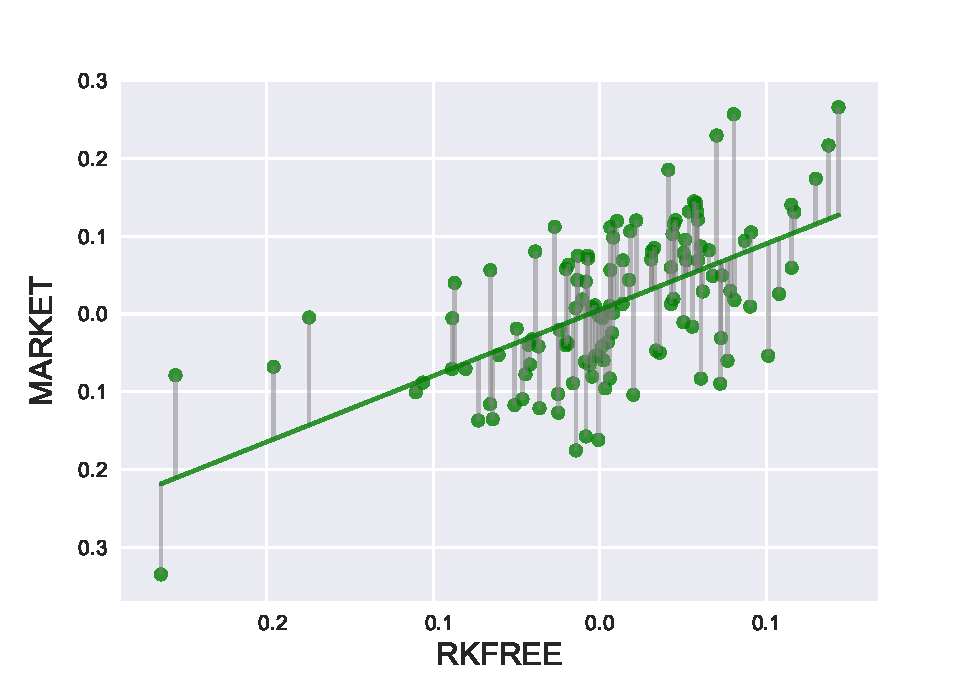
\includegraphics{02-simplereg_files/figure-latex/unnamed-chunk-13-1.pdf}

Строим доверительный интервал.

\begin{Shaded}
\begin{Highlighting}[]
\NormalTok{regr.conf_int()}
\end{Highlighting}
\end{Shaded}

\begin{verbatim}
                  0         1
Intercept -0.009005  0.019511
x          0.640590  1.055709
\end{verbatim}

И проведем F-test.

\begin{Shaded}
\begin{Highlighting}[]
\NormalTok{hypotheses }\OperatorTok{=} \StringTok{'(x = 1)'}
\NormalTok{regr.f_test(r_matrix }\OperatorTok{=}\NormalTok{ hypotheses)}
\end{Highlighting}
\end{Shaded}

\begin{verbatim}
<class 'statsmodels.stats.contrast.ContrastResults'>
<F test: F=array([[2.09891771]]), p=0.1500556415866233, df_denom=118, df_num=1>
\end{verbatim}

Тест Шапиро. Такой же, как и в R. Для удобства можно поместить в табличку.

\begin{Shaded}
\begin{Highlighting}[]
\NormalTok{W, p_value }\OperatorTok{=}\NormalTok{ shapiro(regr.resid)}
\CommentTok{#pd.DataFrame(data = \{'W': [round(W,3)], 'p_value': [round(p_value,3)]\})}
\end{Highlighting}
\end{Shaded}

Генерируем новые данные и строим предсказание.

\begin{Shaded}
\begin{Highlighting}[]
\ImportTok{import}\NormalTok{ random}
\NormalTok{random.seed(}\DecValTok{7}\NormalTok{)}

\NormalTok{newData }\OperatorTok{=}\NormalTok{ df[}\StringTok{'x'}\NormalTok{] }\OperatorTok{+} \FloatTok{0.5}\OperatorTok{*}\NormalTok{np.random.normal(}\BuiltInTok{len}\NormalTok{(df))}
\NormalTok{prediction }\OperatorTok{=}\NormalTok{ regr.predict(newData)}
\end{Highlighting}
\end{Shaded}

А теперь жесть! Построим графички, похожие на autoplot R.

\begin{Shaded}
\begin{Highlighting}[]
\NormalTok{fig_1 }\OperatorTok{=}\NormalTok{ plt.figure(}\DecValTok{1}\NormalTok{)}

\NormalTok{fig_1.axes[}\DecValTok{0}\NormalTok{] }\OperatorTok{=}\NormalTok{ sns.residplot(df[}\StringTok{'x'}\NormalTok{], df[}\StringTok{'y'}\NormalTok{],}
\NormalTok{                                  lowess}\OperatorTok{=}\VariableTok{True}\NormalTok{,}
\NormalTok{                                  scatter_kws}\OperatorTok{=}\NormalTok{\{}\StringTok{'alpha'}\NormalTok{: }\FloatTok{0.6}\NormalTok{\},}
\NormalTok{                                  line_kws}\OperatorTok{=}\NormalTok{\{}\StringTok{'color'}\NormalTok{: }\StringTok{'red'}\NormalTok{, }\StringTok{'lw'}\NormalTok{: }\DecValTok{2}\NormalTok{, }\StringTok{'alpha'}\NormalTok{: }\FloatTok{0.8}\NormalTok{\})}

\NormalTok{fig_1.axes[}\DecValTok{0}\NormalTok{].set_title(}\StringTok{'Residuals vs Fitted'}\NormalTok{)}
\NormalTok{fig_1.axes[}\DecValTok{0}\NormalTok{].set_xlabel(}\StringTok{'Fitted values'}\NormalTok{)}
\NormalTok{fig_1.axes[}\DecValTok{0}\NormalTok{].set_ylabel(}\StringTok{'Residuals'}\NormalTok{)}


\CommentTok{#можем добавить метки потенциальных аутлаеров}
\NormalTok{abs_resid }\OperatorTok{=} \BuiltInTok{abs}\NormalTok{(regr.resid).sort_values(ascending}\OperatorTok{=}\VariableTok{False}\NormalTok{)}
\NormalTok{abs_resid_top3 }\OperatorTok{=}\NormalTok{ abs_resid[:}\DecValTok{3}\NormalTok{]}

\ControlFlowTok{for}\NormalTok{ i }\KeywordTok{in}\NormalTok{ abs_resid_top3.index:}
\NormalTok{    fig_1.axes[}\DecValTok{0}\NormalTok{].annotate(i, }
\NormalTok{                               xy}\OperatorTok{=}\NormalTok{(regr.fittedvalues[i], }
\NormalTok{                                   regr.resid[i]))}
\end{Highlighting}
\end{Shaded}

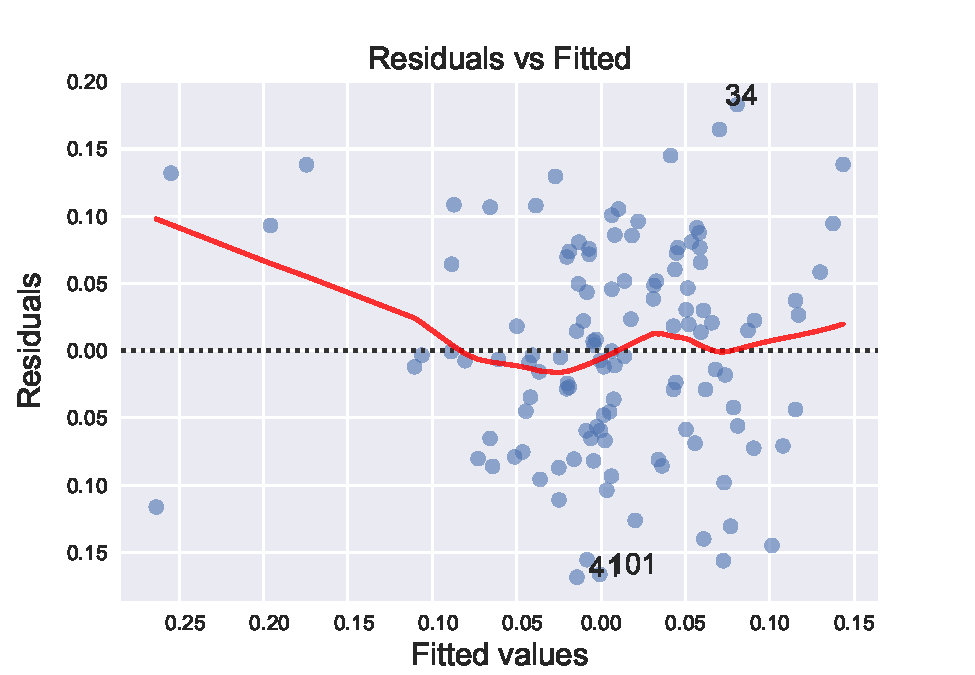
\includegraphics{02-simplereg_files/figure-latex/unnamed-chunk-18-1.pdf}

\begin{Shaded}
\begin{Highlighting}[]
\NormalTok{norm_residuals }\OperatorTok{=}\NormalTok{ regr.get_influence().resid_studentized_internal }\CommentTok{#сохраним стьюдентизированные остатки }


\NormalTok{QQ }\OperatorTok{=}\NormalTok{ gf.ProbPlot(norm_residuals)}
\NormalTok{fig_2 }\OperatorTok{=}\NormalTok{ QQ.qqplot(line}\OperatorTok{=}\StringTok{'45'}\NormalTok{, alpha}\OperatorTok{=}\FloatTok{0.5}\NormalTok{, color}\OperatorTok{=}\StringTok{'b'}\NormalTok{, lw}\OperatorTok{=}\DecValTok{1}\NormalTok{)}


\NormalTok{fig_2.axes[}\DecValTok{0}\NormalTok{].set_title(}\StringTok{'Normal Q-Q'}\NormalTok{)}
\NormalTok{fig_2.axes[}\DecValTok{0}\NormalTok{].set_xlabel(}\StringTok{'Theoretical Quantiles'}\NormalTok{)}
\NormalTok{fig_2.axes[}\DecValTok{0}\NormalTok{].set_ylabel(}\StringTok{'Standardized Residuals'}\NormalTok{)}\OperatorTok{;}

\CommentTok{#и снова метки}
\NormalTok{abs_norm_resid }\OperatorTok{=}\NormalTok{ np.flip(np.argsort(}\BuiltInTok{abs}\NormalTok{(norm_residuals)), }\DecValTok{0}\NormalTok{)}
\NormalTok{abs_norm_resid_top3 }\OperatorTok{=}\NormalTok{ abs_norm_resid[:}\DecValTok{3}\NormalTok{]}

\ControlFlowTok{for}\NormalTok{ r, i }\KeywordTok{in} \BuiltInTok{enumerate}\NormalTok{(abs_norm_resid_top3):}
\NormalTok{    fig_2.axes[}\DecValTok{0}\NormalTok{].annotate(i, }
\NormalTok{                               xy}\OperatorTok{=}\NormalTok{(np.flip(QQ.theoretical_quantiles, }\DecValTok{0}\NormalTok{)[r],}
\NormalTok{                                   norm_residuals[i]))}
\end{Highlighting}
\end{Shaded}

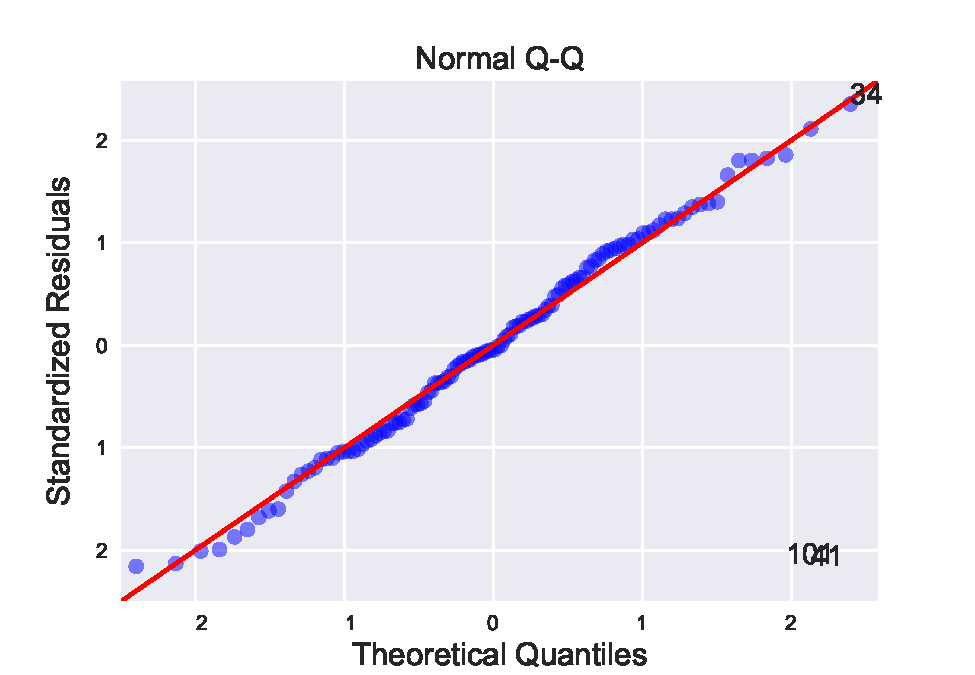
\includegraphics{02-simplereg_files/figure-latex/unnamed-chunk-19-1.pdf}

\begin{Shaded}
\begin{Highlighting}[]
\NormalTok{fig_3 }\OperatorTok{=}\NormalTok{ plt.figure(}\DecValTok{3}\NormalTok{)}

\NormalTok{plt.scatter(regr.fittedvalues, np.sqrt(}\BuiltInTok{abs}\NormalTok{(norm_residuals)), alpha}\OperatorTok{=}\FloatTok{0.5}\NormalTok{)}
\NormalTok{sns.regplot(regr.fittedvalues, np.sqrt(}\BuiltInTok{abs}\NormalTok{(norm_residuals)), }
\NormalTok{            scatter}\OperatorTok{=}\VariableTok{False}\NormalTok{, }
\NormalTok{            ci}\OperatorTok{=}\VariableTok{False}\NormalTok{, }
\NormalTok{            lowess}\OperatorTok{=}\VariableTok{True}\NormalTok{,}
\NormalTok{            line_kws}\OperatorTok{=}\NormalTok{\{}\StringTok{'color'}\NormalTok{: }\StringTok{'red'}\NormalTok{, }\StringTok{'lw'}\NormalTok{: }\DecValTok{1}\NormalTok{, }\StringTok{'alpha'}\NormalTok{: }\FloatTok{0.6}\NormalTok{\})}

\NormalTok{fig_3.axes[}\DecValTok{0}\NormalTok{].set_title(}\StringTok{'Scale-Location'}\NormalTok{)}
\NormalTok{fig_3.axes[}\DecValTok{0}\NormalTok{].set_xlabel(}\StringTok{'Fitted values'}\NormalTok{)}
\NormalTok{fig_3.axes[}\DecValTok{0}\NormalTok{].set_ylabel(}\StringTok{'$\textbackslash{}sqrt\{|Standardized Residuals|\}$'}\NormalTok{)}

\CommentTok{# и еще раз!)}
\NormalTok{abs_sq_norm_resid }\OperatorTok{=}\NormalTok{ np.flip(np.argsort(np.sqrt(}\BuiltInTok{abs}\NormalTok{(norm_residuals)), }\DecValTok{0}\NormalTok{))}
\NormalTok{abs_sq_norm_resid_top3 }\OperatorTok{=}\NormalTok{ abs_sq_norm_resid[:}\DecValTok{3}\NormalTok{]}

\ControlFlowTok{for}\NormalTok{ i }\KeywordTok{in}\NormalTok{ abs_sq_norm_resid_top3:}
\NormalTok{    fig_3.axes[}\DecValTok{0}\NormalTok{].annotate(i, xy}\OperatorTok{=}\NormalTok{(regr.fittedvalues[i], }
\NormalTok{                                   np.sqrt(}\BuiltInTok{abs}\NormalTok{(norm_residuals)[i])))}
\end{Highlighting}
\end{Shaded}

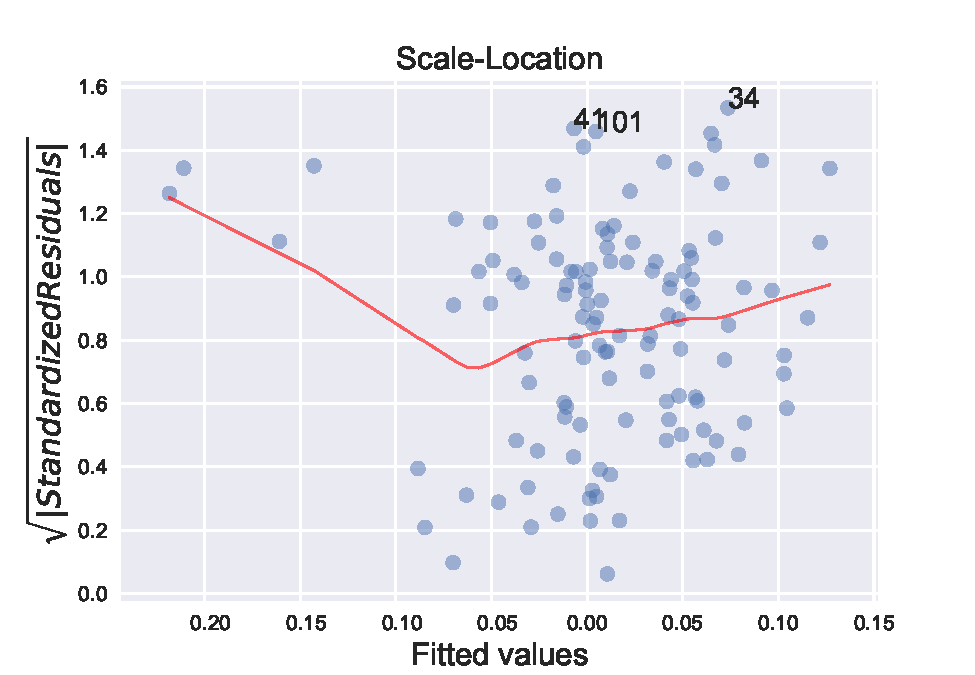
\includegraphics{02-simplereg_files/figure-latex/unnamed-chunk-20-1.pdf}

\begin{Shaded}
\begin{Highlighting}[]
\NormalTok{leverage }\OperatorTok{=}\NormalTok{ regr.get_influence().hat_matrix_diag }\CommentTok{#сохраняем элементы матрицы-шляпницы}
\NormalTok{cook_dist }\OperatorTok{=}\NormalTok{ regr.get_influence().cooks_distance[}\DecValTok{0}\NormalTok{] }\CommentTok{#И расстояние Кука}

\NormalTok{fig_4 }\OperatorTok{=}\NormalTok{ plt.figure(}\DecValTok{4}\NormalTok{)}

\NormalTok{plt.scatter(leverage, norm_residuals, alpha}\OperatorTok{=}\FloatTok{0.5}\NormalTok{)}
\NormalTok{sns.regplot(leverage, norm_residuals, }
\NormalTok{            scatter}\OperatorTok{=}\VariableTok{False}\NormalTok{, }
\NormalTok{            ci}\OperatorTok{=}\VariableTok{False}\NormalTok{, }
\NormalTok{            lowess}\OperatorTok{=}\VariableTok{True}\NormalTok{,}
\NormalTok{            line_kws}\OperatorTok{=}\NormalTok{\{}\StringTok{'color'}\NormalTok{: }\StringTok{'red'}\NormalTok{, }\StringTok{'lw'}\NormalTok{: }\DecValTok{1}\NormalTok{, }\StringTok{'alpha'}\NormalTok{: }\FloatTok{0.8}\NormalTok{\})}

\NormalTok{fig_4.axes[}\DecValTok{0}\NormalTok{].set_xlim(}\DecValTok{0}\NormalTok{, }\FloatTok{0.20}\NormalTok{)}
\end{Highlighting}
\end{Shaded}

\begin{verbatim}
(0, 0.2)
\end{verbatim}

\begin{Shaded}
\begin{Highlighting}[]
\NormalTok{fig_4.axes[}\DecValTok{0}\NormalTok{].set_ylim(}\OperatorTok{-}\DecValTok{3}\NormalTok{, }\DecValTok{5}\NormalTok{)}
\end{Highlighting}
\end{Shaded}

\begin{verbatim}
(-3, 5)
\end{verbatim}

\begin{Shaded}
\begin{Highlighting}[]
\NormalTok{fig_4.axes[}\DecValTok{0}\NormalTok{].set_title(}\StringTok{'Residuals vs Leverage'}\NormalTok{)}
\NormalTok{fig_4.axes[}\DecValTok{0}\NormalTok{].set_xlabel(}\StringTok{'Leverage'}\NormalTok{)}
\NormalTok{fig_4.axes[}\DecValTok{0}\NormalTok{].set_ylabel(}\StringTok{'Standardized Residuals'}\NormalTok{)}


\NormalTok{leverage_top3 }\OperatorTok{=}\NormalTok{ np.flip(np.argsort(cook_dist), }\DecValTok{0}\NormalTok{)[:}\DecValTok{3}\NormalTok{]}

\ControlFlowTok{for}\NormalTok{ i }\KeywordTok{in}\NormalTok{ leverage_top3:}
\NormalTok{    fig_4.axes[}\DecValTok{0}\NormalTok{].annotate(i, }
\NormalTok{                               xy}\OperatorTok{=}\NormalTok{(leverage[i], }
\NormalTok{                                   norm_residuals[i]))}
\NormalTok{plt.show()}
\end{Highlighting}
\end{Shaded}

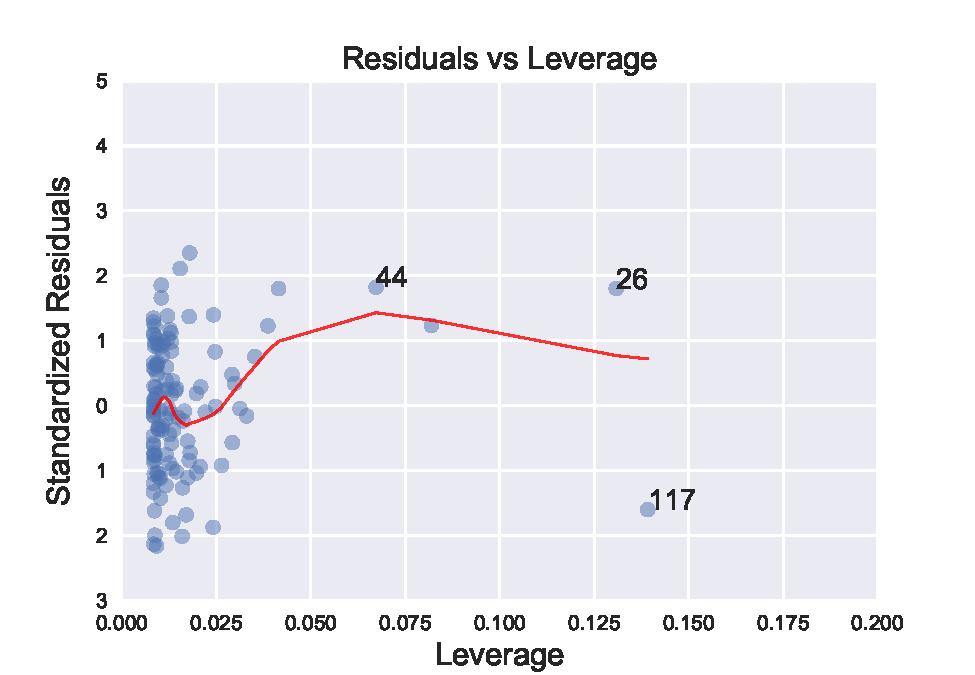
\includegraphics{02-simplereg_files/figure-latex/unnamed-chunk-21-1.pdf}

\bibliography{book.bib,packages.bib}


\end{document}
